\documentclass[11pt,a4paper,]{article}
\usepackage{lmodern}

\usepackage{amssymb,amsmath}
\usepackage{ifxetex,ifluatex}
\usepackage{fixltx2e} % provides \textsubscript
\ifnum 0\ifxetex 1\fi\ifluatex 1\fi=0 % if pdftex
  \usepackage[T1]{fontenc}
  \usepackage[utf8]{inputenc}
\else % if luatex or xelatex
  \usepackage{unicode-math}
  \defaultfontfeatures{Ligatures=TeX,Scale=MatchLowercase}
\fi
% use upquote if available, for straight quotes in verbatim environments
\IfFileExists{upquote.sty}{\usepackage{upquote}}{}
% use microtype if available
\IfFileExists{microtype.sty}{%
\usepackage[]{microtype}
\UseMicrotypeSet[protrusion]{basicmath} % disable protrusion for tt fonts
}{}
\PassOptionsToPackage{hyphens}{url} % url is loaded by hyperref
\usepackage[unicode=true]{hyperref}
\hypersetup{
            pdftitle={Meta-learning how to forecast time series},
            pdfkeywords={Algorithm selection problem, Time series, Random forest, Machine learning interpretability},
            pdfborder={0 0 0},
            breaklinks=true}
\urlstyle{same}  % don't use monospace font for urls
\usepackage{geometry}
\geometry{left=2.5cm,right=2.5cm,top=2.5cm,bottom=2.5cm}
\usepackage[style=authoryear-comp,]{biblatex}
\addbibresource{references.bib}
\usepackage{longtable,booktabs}
% Fix footnotes in tables (requires footnote package)
\IfFileExists{footnote.sty}{\usepackage{footnote}\makesavenoteenv{long table}}{}
\IfFileExists{parskip.sty}{%
\usepackage{parskip}
}{% else
\setlength{\parindent}{0pt}
\setlength{\parskip}{6pt plus 2pt minus 1pt}
}
\setlength{\emergencystretch}{3em}  % prevent overfull lines
\providecommand{\tightlist}{%
  \setlength{\itemsep}{0pt}\setlength{\parskip}{0pt}}
\setcounter{secnumdepth}{5}

% set default figure placement to htbp
\makeatletter
\def\fps@figure{htbp}
\makeatother


\title{Meta-learning how to forecast time series}

%% MONASH STUFF

%% CAPTIONS
\RequirePackage{caption}
\DeclareCaptionStyle{italic}[justification=centering]
 {labelfont={bf},textfont={it},labelsep=colon}
\captionsetup[figure]{style=italic,format=hang,singlelinecheck=true}
\captionsetup[table]{style=italic,format=hang,singlelinecheck=true}

%% FONT
\RequirePackage{bera}
\RequirePackage{mathpazo}

%% HEADERS AND FOOTERS
\RequirePackage{fancyhdr}
\pagestyle{fancy}
\rfoot{\Large\sffamily\raisebox{-0.1cm}{\textbf{\thepage}}}
\makeatletter
\lhead{\textsf{\expandafter{\@title}}}
\makeatother
\rhead{}
\cfoot{}
\setlength{\headheight}{15pt}
\renewcommand{\headrulewidth}{0.4pt}
\renewcommand{\footrulewidth}{0.4pt}
\fancypagestyle{plain}{%
\fancyhf{} % clear all header and footer fields
\fancyfoot[C]{\sffamily\thepage} % except the center
\renewcommand{\headrulewidth}{0pt}
\renewcommand{\footrulewidth}{0pt}}

%% MATHS
\RequirePackage{bm,amsmath}
\allowdisplaybreaks

%% GRAPHICS
\RequirePackage{graphicx}
\setcounter{topnumber}{2}
\setcounter{bottomnumber}{2}
\setcounter{totalnumber}{4}
\renewcommand{\topfraction}{0.85}
\renewcommand{\bottomfraction}{0.85}
\renewcommand{\textfraction}{0.15}
\renewcommand{\floatpagefraction}{0.8}

%\RequirePackage[section]{placeins}

%% SECTION TITLES
\RequirePackage[compact,sf,bf]{titlesec}
\titleformat{\section}[block]
  {\fontsize{15}{17}\bfseries\sffamily}
  {\thesection}
  {0.4em}{}
\titleformat{\subsection}[block]
  {\fontsize{12}{14}\bfseries\sffamily}
  {\thesubsection}
  {0.4em}{}
\titlespacing{\section}{0pt}{*5}{*1}
\titlespacing{\subsection}{0pt}{*2}{*0.2}


%% TITLE PAGE
\def\Date{\number\day}
\def\Month{\ifcase\month\or
 January\or February\or March\or April\or May\or June\or
 July\or August\or September\or October\or November\or December\fi}
\def\Year{\number\year}

\makeatletter
\def\wp#1{\gdef\@wp{#1}}\def\@wp{??/??}
\def\jel#1{\gdef\@jel{#1}}\def\@jel{??}
\def\showjel{{\large\textsf{\textbf{JEL classification:}}~\@jel}}
\def\nojel{\def\showjel{}}
\def\addresses#1{\gdef\@addresses{#1}}\def\@addresses{??}
\def\cover{{\sffamily\setcounter{page}{0}
        \thispagestyle{empty}
        \placefig{2}{1.5}{width=5cm}{monash2}
        \placefig{16.9}{1.5}{width=2.1cm}{MBusSchool}
        \begin{textblock}{4}(16.9,4)ISSN 1440-771X\end{textblock}
        \begin{textblock}{7}(12.7,27.9)\hfill
        
\includegraphics[height=0.7cm]{AACSB}~~~
        
\includegraphics[height=0.7cm]{EQUIS}~~~
        
\includegraphics[height=0.7cm]{AMBA}
        \end{textblock}
        \vspace*{2cm}
        \begin{center}\Large
        Department of Econometrics and Business Statistics\\[.5cm]
        \footnotesize http://monash.edu/business/ebs/research/publications
        \end{center}\vspace{2cm}
        \begin{center}
        \fbox{\parbox{14cm}{\begin{onehalfspace}\centering\Huge\vspace*{0.3cm}
                \textsf{\textbf{\expandafter{\@title}}}\vspace{1cm}\par
                \LARGE\@author\end{onehalfspace}
        }}
        \end{center}
        \vfill
                \begin{center}\Large
                \Month~\Year\\[1cm]
                Working Paper \@wp
        \end{center}\vspace*{2cm}}}
\def\pageone{{\sffamily\setstretch{1}%
        \thispagestyle{empty}%
        \vbox to \textheight{%
        \raggedright\baselineskip=1.2cm
     {\fontsize{24.88}{30}\sffamily\textbf{\expandafter{\@title}}}
        \vspace{2cm}\par
        \hspace{1cm}\parbox{14cm}{\sffamily\large\@addresses}\vspace{1cm}\vfill
        \hspace{1cm}{\large\Date~\Month~\Year}\\[1cm]
        \hspace{1cm}\showjel\vss}}}
\def\blindtitle{{\sffamily
     \thispagestyle{plain}\raggedright\baselineskip=1.2cm
     {\fontsize{24.88}{30}\sffamily\textbf{\expandafter{\@title}}}\vspace{1cm}\par
        }}
\def\titlepage{{\cover\newpage\pageone\newpage\blindtitle}}

\def\blind{\def\titlepage{{\blindtitle}}\let\maketitle\blindtitle}
\def\titlepageonly{\def\titlepage{{\pageone\end{document}}}}
\def\nocover{\def\titlepage{{\pageone\newpage\blindtitle}}\let\maketitle\titlepage}
\let\maketitle\titlepage
\makeatother

%% SPACING
\RequirePackage{setspace}
\spacing{1.5}

%% LINE AND PAGE BREAKING
\sloppy
\clubpenalty = 10000
\widowpenalty = 10000
\brokenpenalty = 10000
\RequirePackage{microtype}

%% PARAGRAPH BREAKS
\setlength{\parskip}{1.4ex}
\setlength{\parindent}{0em}

%% HYPERLINKS
\RequirePackage{xcolor} % Needed for links
\definecolor{darkblue}{rgb}{0,0,.6}
\RequirePackage{url}

\makeatletter
\@ifpackageloaded{hyperref}{}{\RequirePackage{hyperref}}
\makeatother
\hypersetup{
     citecolor=0 0 0,
     breaklinks=true,
     bookmarksopen=true,
     bookmarksnumbered=true,
     linkcolor=darkblue,
     urlcolor=blue,
     citecolor=darkblue,
     colorlinks=true}

%% KEYWORDS
\newenvironment{keywords}{\par\vspace{0.5cm}\noindent{\sffamily\textbf{Keywords:}}}{\vspace{0.25cm}\par\hrule\vspace{0.5cm}\par}

%% ABSTRACT
\renewenvironment{abstract}{\begin{minipage}{\textwidth}\parskip=1.4ex\noindent
\hrule\vspace{0.1cm}\par{\sffamily\textbf{\abstractname}}\newline}
  {\end{minipage}}


\usepackage[T1]{fontenc}
\usepackage[utf8]{inputenc}

\usepackage[showonlyrefs]{mathtools}
\usepackage[no-weekday]{eukdate}

%% BIBLIOGRAPHY

\makeatletter
\@ifpackageloaded{biblatex}{}{\usepackage[style=authoryear-comp, backend=biber, natbib=true]{biblatex}}
\makeatother
\ExecuteBibliographyOptions{bibencoding=utf8,minnames=1,maxnames=3, maxbibnames=99,dashed=false,terseinits=true,giveninits=true,uniquename=false,uniquelist=false,doi=false, isbn=false,url=true,sortcites=false}

\DeclareFieldFormat{url}{\texttt{\url{#1}}}
\DeclareFieldFormat[article]{pages}{#1}
\DeclareFieldFormat[inproceedings]{pages}{\lowercase{pp.}#1}
\DeclareFieldFormat[incollection]{pages}{\lowercase{pp.}#1}
\DeclareFieldFormat[article]{volume}{\mkbibbold{#1}}
\DeclareFieldFormat[article]{number}{\mkbibparens{#1}}
\DeclareFieldFormat[article]{title}{\MakeCapital{#1}}
\DeclareFieldFormat[inproceedings]{title}{#1}
\DeclareFieldFormat{shorthandwidth}{#1}
% No dot before number of articles
\usepackage{xpatch}
\xpatchbibmacro{volume+number+eid}{\setunit*{\adddot}}{}{}{}
% Remove In: for an article.
\renewbibmacro{in:}{%
  \ifentrytype{article}{}{%
  \printtext{\bibstring{in}\intitlepunct}}}

\makeatletter
\DeclareDelimFormat[cbx@textcite]{nameyeardelim}{\addspace}
\makeatother
\renewcommand*{\finalnamedelim}{%
  %\ifnumgreater{\value{liststop}}{2}{\finalandcomma}{}% there really should be no funny Oxford comma business here
  \addspace\&\space}


\wp{no/yr}
\jel{C10,C14,C22}

\RequirePackage[absolute,overlay]{textpos}
\setlength{\TPHorizModule}{1cm}
\setlength{\TPVertModule}{1cm}
\def\placefig#1#2#3#4{\begin{textblock}{.1}(#1,#2)\rlap{\includegraphics[#3]{#4}}\end{textblock}}



\blind



\date{\sf\Date~\Month~\Year}
\makeatletter
 \lfoot{\sf\@date}
\makeatother

%% Any special functions or other packages can be loaded here.
%% Any special functions or other packages can be loaded here.
\usepackage{algorithm}
\usepackage{algpseudocode}
\usepackage{amsthm}
\usepackage{amsmath,bm}
\usepackage{paralist}
\usepackage{todonotes}
\usepackage{ctable}
\usepackage{float}
\usepackage{tikz}
\usepackage{algorithm}
\usepackage{multirow}
\usepackage{lscape}
\usepackage{rotating}
\usepackage{bm} 
\usepackage{threeparttable}
\floatplacement{figure}{H} 

\def\sectionautorefname{Section}
\captionsetup[figure]{font=small}
\captionsetup[table]{font=small}
\def\var{\text{Var}}
\allowdisplaybreaks
\sloppy

%% LINE AND PAGE BREAKING
\clubpenalty = 4500
\widowpenalty = 4500
\brokenpenalty = 4500


\def\yes{$\checkmark$}

\setlength{\abovedisplayskip}{5pt}
\setlength{\belowdisplayskip}{5pt}
\setlength{\abovedisplayshortskip}{0pt}
\setlength{\belowdisplayshortskip}{0pt}


\begin{document}
\maketitle
\begin{abstract}
Features of time series are useful in identifying suitable models for forecasting. We present a general framework, labelled FFORMS (Feature-based FORecast Model Selection), which selects forecast models based on features calculated from the time series. The FFORMS framework builds a mapping that relates the features of a time series to the ``best'' forecast model using a random forest. The framework is evaluated using time series from the M1 and M3 competitions and is shown to yield accurate forecasts comparable to several benchmarks and other commonly used automated approaches of time series forecasting. Furthermore, we explore what is happening under the hood of the FFORMS framework. This is accomplished using model-agnostic machine learning interpretability approaches. The analysis provides a valuable insight into how different features and their interactions affect the choice of forecast model.
\end{abstract}
\begin{keywords}
Algorithm selection problem, Time series, Random forest, Machine learning interpretability
\end{keywords}

\hypertarget{introduction}{%
\section{Introduction}\label{introduction}}

Forecasting is a key activity for any business to operate efficiently. The rapid advances in computing technologies have enabled businesses to keep track of large numbers of time series. Hence, it is becoming increasingly common to have to regularly forecast many millions of time series. For example, large scale businesses may be interested in forecasting sales, cost, and demand for their thousands of products across various locations, warehouses, etc. Technology companies such as Google collect many millions of daily time series such as web-click logs, web search counts, queries, revenues, number of users for different services, etc. Such large collections of time series require fast automated procedures generating accurate forecasts. The scale of these tasks has raised some computational challenges we seek to address by proposing a new fast algorithm for model selection and time series forecasting.

Two alternative strategies for generating such a large number of forecasts are: (1) to either use a single forecasting method across all the time series; or (2) to select an appropriate forecasting method for each time series individually. It is highly unlikely that a single method will consistently outperform judiciously chosen competitor methods across all time series. We therefore reject the former strategy and focus on an approach for selecting an individual forecasting method for each time series.

Selecting the most appropriate model for forecasting a given time series can be challenging. Two of the most commonly used automated algorithms are the exponential smoothing (\texttt{ets}) algorithm of \textcite{Hyndman2002} and the ARIMA (\texttt{auto.arima}) algorithm of \textcite{Hyndman2008}. Both algorithms are implemented in the forecast package in R \autocites{Rcore}{forecast}. In this paradigm, a class of models is selected in advance, and many models within that class are estimated for each time series. The model with the smallest AICc value is chosen and used for forecasting. This approach relies on the expert judgement of the forecaster in first selecting the most appropriate class of models to use, as it is not usually possible to compare AICc values between model classes due to differences in the way the likelihood is computed, and the way initial conditions are handled.

An alternative approach, which avoids selecting a class of models \emph{a priori}, is to use a simple ``hold-out'' test set; but then there is often insufficient data to draw a reliable conclusion. To overcome this drawback, time series cross-validation can be used \autocite{hyndman2014forecasting}; then models from many different classes may be applied, and the model with the lowest cross-validated MSE selected. However, this increases the computation time involved considerably (at least to order \(n^2\) where \(n\) is the number of series to be forecast).

Clearly, there is a need for a fast and scalable algorithm to automate the process of selecting models with the aim of forecasting.
There have been several recent studies on the use of meta-learning approaches to automate forecast model selection based on features computed from the time series \autocites{shah1997model}{prudencio2004meta}{lemke2010meta}{kuck2016meta}. A meta-learning approach provides systematic guidance on model selection based on knowledge acquired from historical data sets. The key idea is that forecast model selection is posed as a supervised learning task. Each time series in the metadata set is represented as a vector of features and labelled according to the best forecast model (for example, the model with the lowest mean absolute scaled error (MASE) over a test set). Then a meta-learner is trained to identify a suitable forecast model (usually a machine learning algorithm is used). In the era of big data, such an automated model selection process is necessary because the cost of invoking all possible forecast models is prohibitive. However, the existing literature suffers from limited answers to questions such as: How are features related to the property being modelled? How do features interact with each other to identify a suitable forecast model? Which features contribute most to the classification process? Addressing such questions can enhance the understanding of the relations between features and model selection outcomes. To the best of our knowledge, a very limited effort has been made to understand how the meta-learners are making their decisions and what is really happening inside these complex model structures. Providing transparency will result, building trust in the prediction results of the meta-learner.

We propose a general meta-learning framework using features of the time series to select the class of models, or even the specific model, to be used for forecasting. We refer to this general framework as FFORMS (\textbf{F}eature-based \textbf{FOR}ecast-\textbf{M}odel \textbf{S}election). The forecast model selection process is carried out using a classification algorithm --- we use the time series features as inputs, and the ``best'' forecasting model as the output. A random forest is used to model the relationship between features and best performing forecast model. The classifier is built using a large historical collection of time series, in advance of the forecasting task at hand. Hence, this is an ``offline'' procedure. The ``online'' process of generating forecasts only involves calculating the features of a time series and using the pre-trained classifier to identify the best forecasting model. Hence, generating forecasts only involves the estimation of a single forecasting model, with no need to estimate large numbers of models within a class, or to carry out a computationally-intensive cross-validation procedure. To fill the gaps in the literature, this paper makes a first step towards providing a comprehensive analysis of the relationship between time series features and forecast model selection using machine learning interpretability techniques.

In this article, we make the following contributions:

\begin{enumerate}
\def\labelenumi{\arabic{enumi}.}
\item
  We explore the use of random forest algorithm to model the relationship between time series features and the `best' forecast model. The motivation behind the use of random forest classifiers are: i) it can model complex interactions between features; ii) the modelling framework captures linear and non-linear effects of features through the averaging of large number of decision trees; iii) its robustness against over-fitting the training data; iv) it is easy to handle the problem of imbalanced classes; v) it is a fast approach compared to boosting algorithms and vi) it is fairly easy and straightforward to implement with available software. The contribution of this paper differs from previously published work related to meta-learning \autocites{prudencio2004meta}{lemke2010meta}{kuck2016meta} in three ways: i) a more extensive collection of features is used (features to handle multiple seasonality in hourly and daily series), ii) the diversity of forecast models considered class labels, and iii) the capability of handling high frequency data.
\item
  The second contribution of the paper is the exploration of what is happening under the hood of the FFORMS framework, leading to an understanding of the relationship between features of time series and the choice of forecast model selection using the FFORMS framework. We call it `Peeking inside FFORMS'. We try to answer the following questions:

  \begin{enumerate}
  \def\labelenumii{\roman{enumii})}
  \tightlist
  \item
    \textbf{Which} features are the most important?
  \item
    \textbf{Where} (overall classification or only within specific classes) are they important?
  \item
    \textbf{How} are they important?
  \item
    \textbf{When} and \textbf{how} are features linked to the prediction outcome?
  \item
    \textbf{When} and \textbf{how strongly} do features interact with other features?
  \end{enumerate}
\end{enumerate}

The remainder of the paper is structured as follows. The \autoref{fforms} outlines the extended FFORMS framework. \autoref{offline} through \autoref{peeking} explain the three main components of the extended FFORMS framework. Results are discussed in \autoref{results1} and \autoref{results2}. \autoref{conclusions} concludes.

\hypertarget{litreview}{%
\section{Literature review}\label{litreview}}

\hypertarget{time-series-features}{%
\subsection{Time series features}\label{time-series-features}}

Rather than work with the time series directly at the level of individual observations, we propose analysing time series via an associated ``feature space''. A time series feature is any measurable characteristic of a time series. For example, \autoref{fig:fig1} shows the time-domain representation of six time series taken from the M3 competition \autocite{makridakis2000m3} while \autoref{fig:fig2} shows a feature-based representation of the same time series. Here only two features are considered: the strength of seasonality and the strength of trend, calculated based on the measures introduced by \textcite{wang2009rule}. Time series in the lower right quadrant of \autoref{fig:fig2} are non-seasonal but trended, while there is only one series with both high trend and high seasonality. We also see how the degree of seasonality and trend varies between series. Other examples of time series features include autocorrelation, spectral entropy and measures of self-similarity and nonlinearity. \textcite{fulcher2014highly} identified 9000 operations to extract features from time series.

\begin{figure}

{\centering 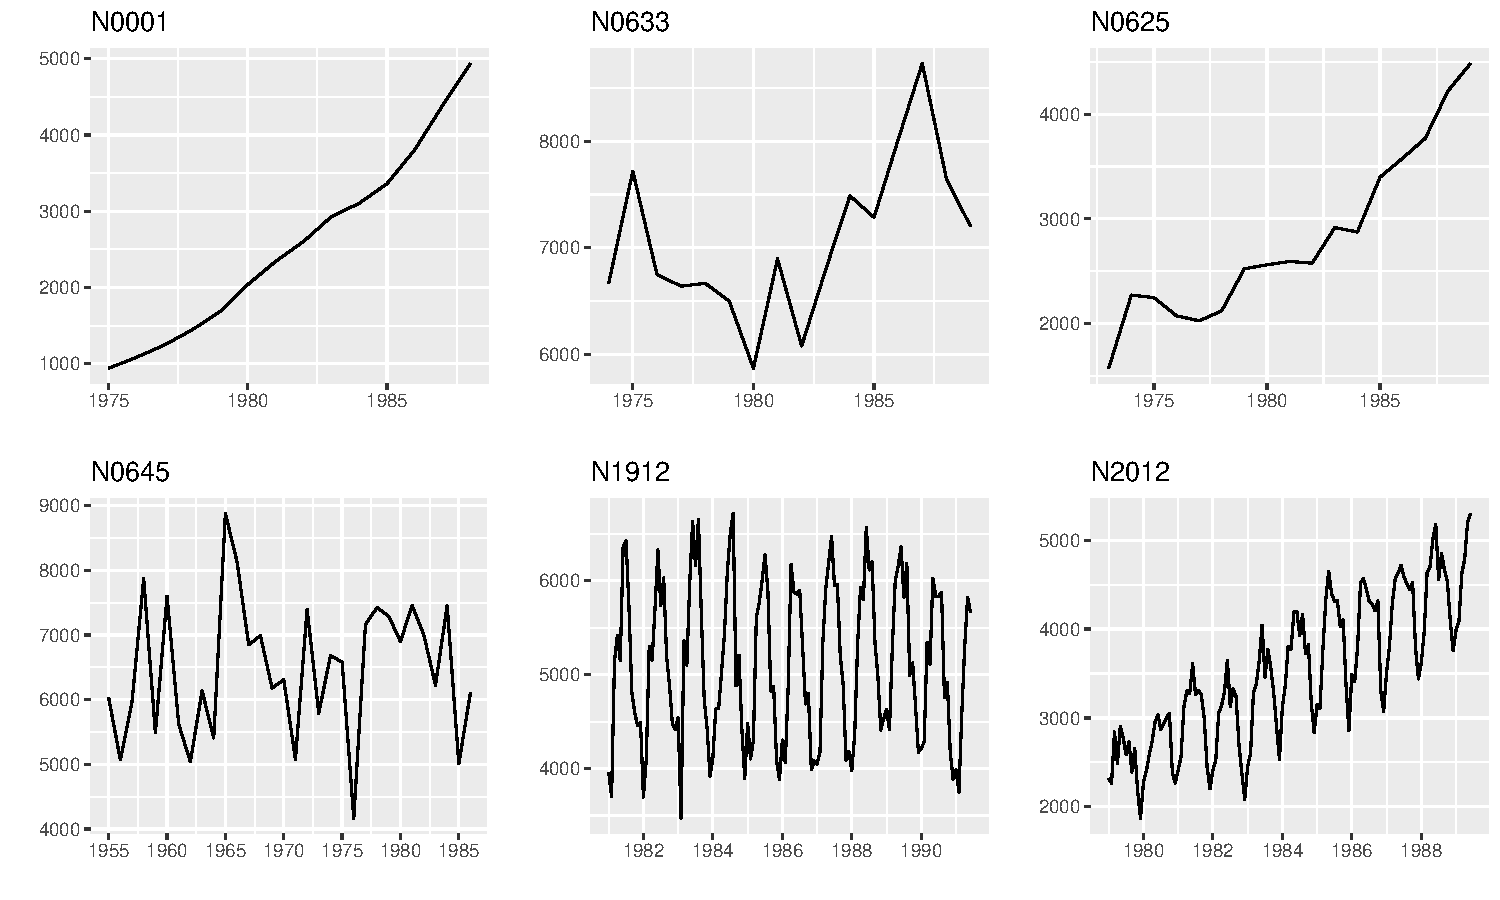
\includegraphics[width=\textwidth]{figure/fig1-1} 

}

\caption{Time-domain representation of time series}\label{fig:fig1}
\end{figure}

\begin{figure}

{\centering 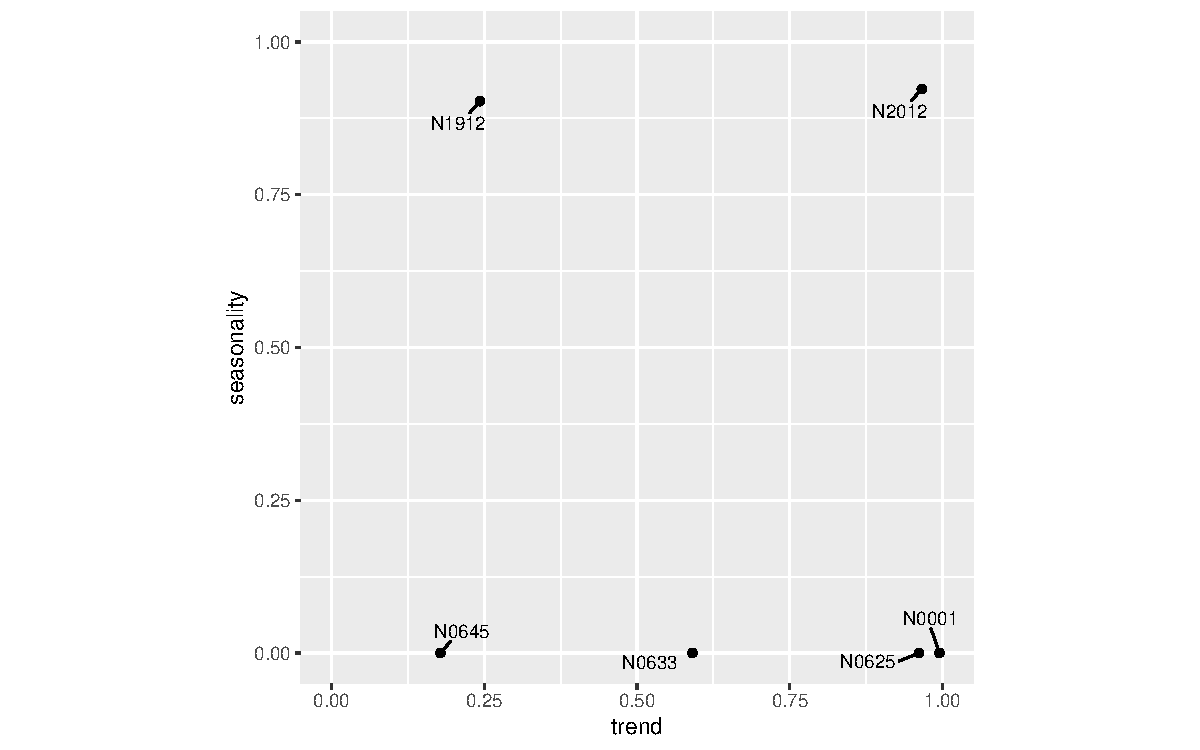
\includegraphics[width=0.7\linewidth]{figure/fig2-1} 

}

\caption{Feature-based representation of time series}\label{fig:fig2}
\end{figure}

\hypertarget{meta-learning-for-algorithm-selection}{%
\subsection{Meta-learning for algorithm selection}\label{meta-learning-for-algorithm-selection}}

John Rice was an early and strong proponent of the idea of meta-learning, which he called the algorithm selection problem (ASP) \autocite{rice1976}. The term \emph{meta-learning} started to appear with the emergence of the machine-learning literature. Rice's framework for algorithm selection is shown in \autoref{fig:rice} and comprises four main components. The problem space, \(P\), represents the data sets used in the study. The feature space, \(F\), is the range of measures that characterize the problem space \(P\). The algorithm space, \(A\), is a list of suitable candidate algorithms which can be used to find solutions to the problems in \(P\). The performance metric, \(Y\), is a measure of algorithm performance such as accuracy, speed, etc. A formal definition of the algorithm selection problem is given by \textcite{smith2009cross}, and repeated below.

\begin{quote}
\textbf{Algorithm selection problem}. For a given problem instance \(x \in P\), with features \(f(x) \in F\), find the selection mapping \(S(f(x))\) into algorithm space \(A\), such that the selected algorithm \(\alpha \in A\) maximizes the performance mapping \(y(\alpha(x)) \in Y\).
\end{quote}

\begin{figure}

{\centering 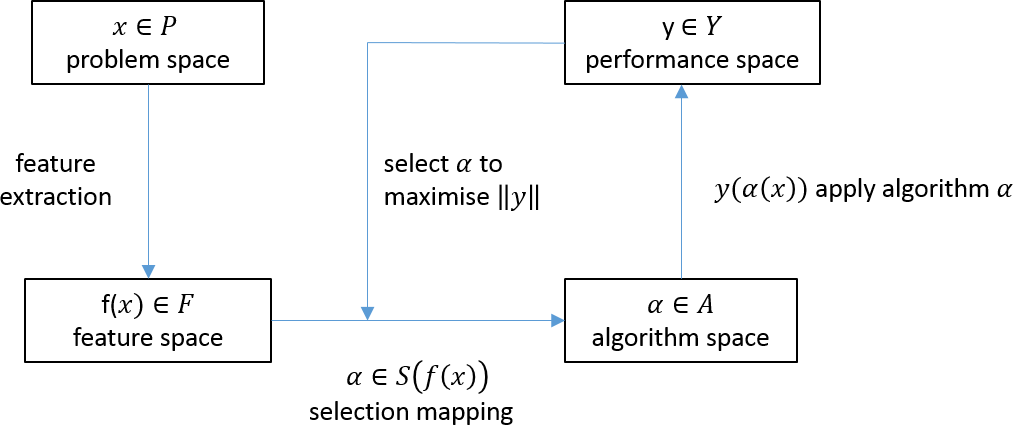
\includegraphics[width=0.8\linewidth]{images/RiceFramework} 

}

\caption{Rice's framework for the Algorithm Selection Problem.}\label{fig:rice}
\end{figure}

The main challenge in ASP is to identify the selection mapping \(S\) from the feature space to the algorithm space. Even though Rice's framework articulates a conceptually rich framework, it does not specify how to obtain \(S\). This gives rise to the meta-learning approach.

\hypertarget{forecast-model-selection-using-meta-learning}{%
\subsection{Forecast-model selection using meta-learning}\label{forecast-model-selection-using-meta-learning}}

Selecting models for forecasting can be framed according to Rice's ASP framework.

\begin{quote}
\textbf{Forecast-model selection problem}. For a given time series \(x \in P\), with features \(f(x) \in F\), find the selection mapping \(S(f(x))\) into the algorithm space \(A\), such that the selected algorithm \(\alpha \in A\) minimizes forecast accuracy error metric \(y(\alpha(x)) \in Y\) on the test set of the time series.
\end{quote}

Existing methods differ with respect to the way they define the problem space (\(A\)), the features (\(F\)), the forecasting accuracy measure (\(Y\)) and the selection mapping (\(S\)).

\textcite{collopy1992rule} introduced 99 rules based on 18 features of time series, in order to make forecasts for economic and demographic time series. This work was extended by \textcite{armstrong2001s} to reduce human intervention.

\textcite{shah1997model} used the following features to classify time series: the number of observations, the ratio of the number of turning points to the length of the series, the ratio of number of step changes, skewness, kurtosis, the coefficient of variation, autocorrelations at lags 1--4, and partial autocorrelations at lag 2--4. Casting Shah's work in Rice's framework, we can specify: \(P=203\) quarterly series from the M1 competition \autocite{makridakis1982accuracy}; \(A=3\) forecasting methods, namely simple exponential smoothing, Holt-Winters exponential smoothing with multiplicative seasonality, and a basic structural time series model; \(Y=\) mean squared error for a hold-out sample. \textcite{shah1997model} learned the mapping \(S\) using discriminant analysis.

\textcite{prudencio2004meta} was the first paper to use the term ``meta-learning'' in the context of time series model selection. They studied the applicability of meta-learning approaches for forecast-model selection based on two case studies. Again using the notation above, we can describe their first case study with: \(A\) contained only two forecasting methods, simple exponential smoothing and a time-delay neural network; \(Y=\) mean absolute error; \(F\) consisted of 14 features, namely length, autocorrelation coefficients, coefficient of variation, skewness, kurtosis, and a test of turning points to measure the randomness of the time series; \(S\) was learned using the C4.5 decision tree algorithm. For their second study, the algorithm space included a random walk, Holt's linear exponential smoothing and AR models; the problem space \(P\) contained the yearly series from the M3 competition \autocite{makridakis2000m3}; \(F\) included a subset of features from the first study; and \(Y\) was a ranking based on error. Beyond the task of forecast-model selection, they used the NOEMON approach to rank the algorithms \autocite{kalousis1999noemon}.

\textcite{lemke2010meta} studied the applicability of different meta-learning approaches for time series forecasting. Their algorithm space \(A\) contained ARIMA models, exponential smoothing models and a neural network model. In addition to statistical measures such as the standard deviation of the de-trended series, skewness, kurtosis, length, strength of trend, Durbin-Watson statistics of regression residuals, the number of turning points, step changes, a predictability measure, nonlinearity, the largest Lyapunov exponent, and auto-correlation and partial-autocorrelation coefficients, they also used frequency domain based features. The feed forward neural network, decision tree and support vector machine approaches were considered to learn the mapping \(S\).

\textcite{wang2009rule} used a meta-learning framework to provide recommendations as to which forecast method to use to generate forecasts. In order to evaluate forecast accuracy, they introduced a new measure \(Y =\) \emph{simple percentage better (SPB)}, which calculates the forecasting accuracy of a method against the forecasting accuracy error of random walk model. They used a feature set \(F\) comprising nine features: strength of trend, strength of seasonality, serial correlation, nonlinearity, skewness, kurtosis, self-similarity, chaos and periodicity. The algorithm space \(A\) included eight forecast-models, namely, exponential smoothing, ARIMA, neural networks and random walk model; while the mapping \(S\) was learned using the C4.5 algorithm for building decision trees. In addition, they used SOM clustering on the features of the time series in order to understand the nature of time series in a two-dimensional setting.

The set of features introduced by \textcite{wang2009rule} was later used by \textcite{widodomodel} to develop a meta-learning framework for forecast-model selection. The authors further reduced the dimensionality of time series by performing principal component analysis on the features.

More recently, \textcite{kuck2016meta} proposed a meta-learning framework based on neural networks for forecast-model selection. Here, \(P = 78\) time series from the NN3 competition were used to build the meta-learner. They introduced a new set of features based on forecasting errors. The average symmetric mean absolute percentage error was used to identify the best forecast-models for each series. They classify their forecast-models in the algorithm space \(A\), comprising single, seasonal, seasonal-trend and trend exponential smoothing. The mapping \(S\) was learned using a feed-forward neural network. Further, they evaluated the performance of different sets of features for forecast-model selection.

\hypertarget{methodology}{%
\section{Methodology}\label{methodology}}

Our proposed FFORMS framework, presented in \autoref{fig:framework}, builds on this preceding research. The offline and online phases are shown in blue and red respectively. A classification algorithm (the meta-learner) is trained during the offline phase and is then used to select an appropriate forecast model for a new time series in the online phase. Furthermore, we use machine learning interpretability tools to gain insights into what is happening under the hood of the FFORMS framework. We refer to this process as ``peeking inside FFORMS'' which is shown in yellow.

\begin{figure}

{\centering 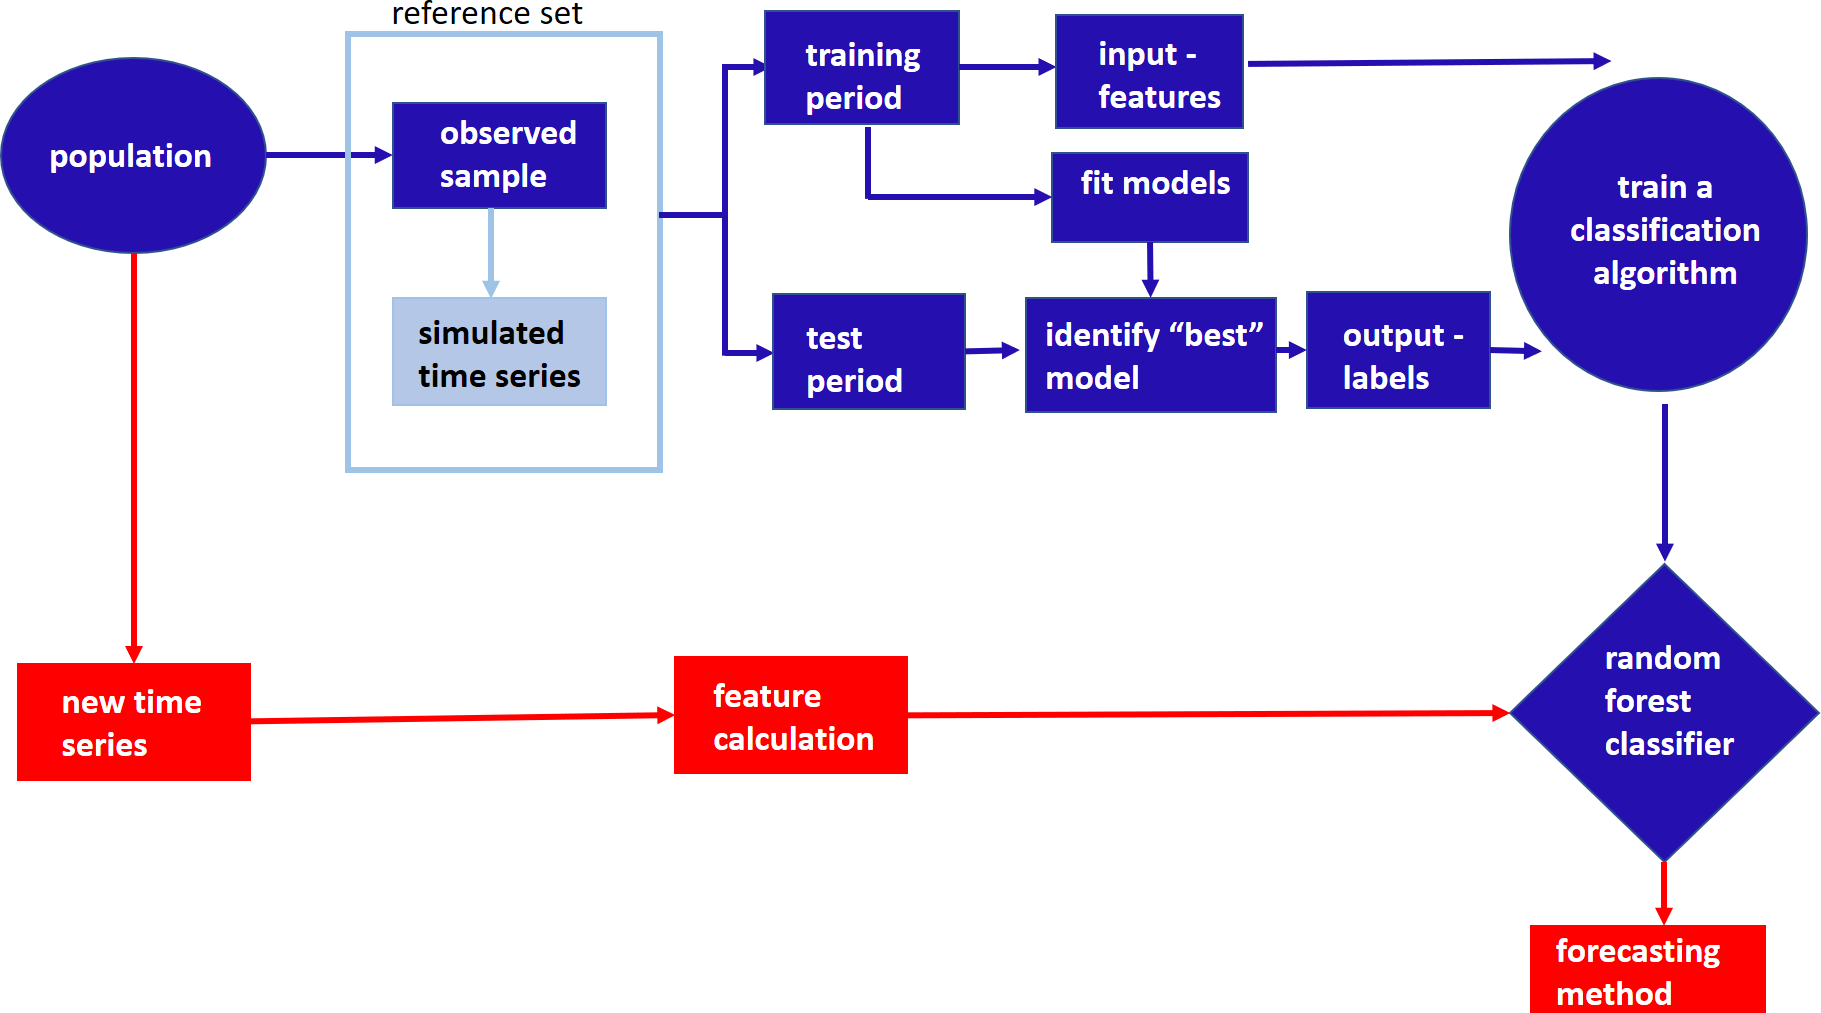
\includegraphics[width=1.1\linewidth]{images/framework} 

}

\caption{FFORMS (Feature-based FORecast-Model Selection) framework. The offline phase is shown in blue, the online phase in red and the peeking inside FFORMS is shown in yellow.}\label{fig:framework}
\end{figure}

In order to train our classification algorithm, we need a large collection of time series which are similar to those we will be forecasting. We assume that we have an essentially infinite population of time series, and we take a sample of them in order to train the classification algorithm denoted as the ``observed sample''. The new time series we wish to forecast can be thought of as additional draws from the same population. Hence, any conclusions made from the classification framework refer only to the population from which the sample has been selected. We may call this the ``target population'' of time series. It is important to have a well-defined target population to avoid misapplying the classification rules. In practice, we may wish to augment the set of observed time series by simulating new time series similar to those in the assumed population (we provide details and discussion in Section \ref{simulatingseries} that follows). We denote the total collection of time series used for training the classifier as the ``reference set''.
Each time series within the reference set is split into a training period and a test period. From each training period we compute a range of time series features, and fit a selection of candidate models. The calculated features form the input vector to the classification algorithm. Using the fitted models, we generate forecasts and identify the ``best'' model for each time series based on a forecast error measure (e.g., MASE) calculated over the test period. The models deemed ``best'' form the output labels for the classification algorithm. The pseudo code for our proposed framework is presented in Algorithm \ref{alg:algo-lab} below. In the following sections, we briefly discuss aspects of the offline phase.

\begin{algorithm}[!ht]
  \caption{The FFORMS framework - Forecasting based on meta-learning. }
  \label{alg:algo-lab}
  \begin{algorithmic}[1]
    \Statex \textbf{Offline phase - train the classifier}
    \Statex \text{Given:}
    \Statex \hspace{1cm}$O=\{x_1, x_2, \dots,x_n\}:$ the collection of $n$ observed time series.
      \Statex \hspace{1cm}$L:$ the set of class labels (e.g.\ ARIMA, ETS, SNAIVE).
         \Statex \hspace{1cm}$F:$ the set of functions to calculate time series features.
         \Statex \hspace{1cm}$nsim:$ number of series to be simulated.
         \Statex \hspace{1cm}$B:$ number of trees in the random forest.
         \Statex \hspace{1cm}$k:$ number of features to be selected at each node.
     \Statex \text{Output:}
      \Statex \hspace{1cm}\text{FFORMS classifier}
      \Statex
     \Statex \textit{Prepare the reference set}
    \Statex For $i=1$ to $n$:
            \State Fit ARIMA and ETS models to $x_i$.
            \State Simulate $nsim$ time series from each model in step 1.
            \State The time series in $O$ and simulated time series in step 2 form the reference set $R=\{x_1, x_2, \dots,x_n, x_{n+1},\dots,x_N\}$ where $N = n + nsim$.
    \Statex
    \Statex \textit{Prepare the meta-data}
    \Statex For $j=1$ to $N$:
            \State Split $x_j$ into a training period and test period.
            \State Calculate features $F$ based on the training period.
            \State Fit $L$ models to the training period.
            \State Calculate forecasts for the test period from each model.
            \State Calculate forecast error measure over the test period for all models in $L$.
            \State Select the model with the minimum forecast error.
            \State Meta-data: input features (step 5), output labels (step 9).
     \Statex
    \Statex \textit{Train a random forest classifier}
            \State Train a random forest classifier based on the meta-data.
            \State {Random forest: the ensemble of trees $\{T_b\}_1^B$}.
    \Statex
     \Statex \textbf{Online phase - forecast a new time series}
    \Statex \text{Given:}
    \Statex \hspace{1cm}\text{FFORMS classifier from step 12} .
     \Statex \text{Output:}
      \Statex \hspace{1cm}\text{class labels for new time series $x_{new}$}.
  \State For $x_{new}$ calculate features $F$.
  \State Let $\hat{C_b}(x_{new})$ be the class prediction of the $b^{th}$ random forest tree. Then class label for $x_{new}$ is $\hat{C_{rf}}(x_{new})=majorityvote\{\hat{C_b}(x_{new})\}_1^B$.
   \end{algorithmic}
\end{algorithm}

\hypertarget{simulatingseries}{%
\subsection{Augmenting the observed sample with simulated time series}\label{simulatingseries}}

In practice, we may wish to augment the set of observed time series by simulating new time series similar to those in the assumed population. This process may be useful when the number of observed time series is too small to build a reliable classifier. Alternatively, we may wish to add more of some particular types of time series to the reference set in order to get a more balanced sample for the classification. In order to produce simulated series that are similar to those in the population, we consider two classes of data generating processes: exponential smoothing models and ARIMA models. Using the automated \texttt{ets} and \texttt{auto.arima} algorithms \autocite{forecast} we identify models, based on model selection criteria (such as AICc) and simulate multiple time series from the selected models within each model class. Assuming the models produce data that are similar to the observed time series ensures that the simulated series are similar to those in the population. As this is done in the offline phase of the algorithm the computational time in producing these simulated series is of no real consequence.

\hypertarget{input-features}{%
\subsection{Input: features}\label{input-features}}

Our proposed FFORMS algorithm requires features that enable identification of a suitable forecast model for a given time series. Therefore, the features used should capture the dynamic structure of the time series, such as trend, seasonality, autocorrelation, nonlinearity, heterogeneity, and so on. Furthermore, interpretability, robustness to outliers, scale and length independence should also be considered when selecting features for this classification problem. A comprehensive description of the features used in the experiment is presented in \autoref{feature}.

A feature of the proposed FFORMS framework is that its online phase is fast compared to the time required for implementing a typical model selection or cross-validation procedure. Therefore, we consider only features that can be computed rapidly, as this computation must be done during the online phase.

\begin{table}[!htp]
\centering\footnotesize\tabcolsep=0.12cm
\caption{Time series features}
\label{feature}
\begin{tabular}{llp{8,8cm}cccc}
\toprule
\multicolumn{2}{c}{Feature} & Description & Y & Q/M & W & D/H\\
\midrule
1  & T              & length of time series                                                                   & \yes  & \yes & \yes & \yes\\
2  & trend          & strength of trend                                                                       & \yes  & \yes & \yes & \yes\\
3  & seasonality\_q    & strength of quarterly seasonality                                                    & -     & \yes & - & -\\
4  & seasonality\_m    & strength of monthly seasonality                                                      & -     & \yes & - & -\\
5  & seasonality\_w    & strength of weekly seasonality                                                       & -     & - & \yes & \yes \\
6  & seasonality\_d    & strength of daily seasonality                                                        & -     & - & - & \yes\\
7  & seasonality\_y    & strength of yearly seasonality                                                       & -     & - & - & \yes\\
8  & linearity      & linearity                                                                               & \yes  & \yes & \yes & \yes\\
9  & curvature      & curvature                                                                               & \yes  & \yes & \yes & \yes\\
10  & spikiness      & spikiness                                                                               & \yes  & \yes & \yes & \yes\\
11  & e\_acf1        & first ACF value of remainder series                                                     & \yes  & \yes & \yes & \yes\\
12  & stability      & stability                                                                               & \yes  & \yes & \yes & \yes\\
13  & lumpiness      & lumpiness                                                                               & \yes  & \yes & \yes & \yes\\
14 & entropy        & spectral entropy                                                                        & \yes  & \yes & \yes & \yes\\
15 & hurst          & Hurst exponent                                                                          & \yes  & \yes & \yes & \yes\\
16 & nonlinearity   & nonlinearity                                                                            & \yes\ & \yes & \yes & \yes\\
17 & alpha          & ETS(A,A,N) $\hat\alpha$                                                                 & \yes  & \yes & \yes & -\\
18 & beta           & ETS(A,A,N) $\hat\beta$                                                                  & \yes  & \yes & \yes & - \\
19 & hwalpha        & ETS(A,A,A) $\hat\alpha$                                                                 & -     & \yes & - & -\\
20 & hwbeta         & ETS(A,A,A) $\hat\beta$                                                                  & -     & \yes & - & - \\
21 & hwgamma        & ETS(A,A,A) $\hat\gamma$                                                                 & -     & \yes & - &-\\
22 & ur\_pp         & test statistic based on Phillips-Perron test                                            & \yes  & - & - & - \\
23 & ur\_kpss       & test statistic based on KPSS test                                                       & \yes  & - & - & - \\
24 & y\_acf1        & first ACF value of the original series                                                  & \yes  & \yes & \yes & \yes\\
25 & diff1y\_acf1   & first ACF value of the differenced series                                               & \yes  & \yes & \yes & \yes\\
26 & diff2y\_acf1   & first ACF value of the twice-differenced series                                         & \yes  & \yes & \yes & \yes\\
27 & y\_acf5        & sum of squares of first 5 ACF values of original series                                 & \yes  & \yes & \yes & \yes\\
28 & diff1y\_acf5   & sum of squares of first 5 ACF values of differenced series                              & \yes  & \yes & \yes & \yes\\
29 & diff2y\_acf5   & sum of squares of first 5 ACF values of twice-differenced series                        & \yes  & \yes & \yes & \yes \\
30 & sediff\_acf1 & ACF value at the first lag of seasonally-differenced series                               & -     & \yes & \yes & \yes\\
31 & sediff\_seacf1 & ACF value at the first seasonal lag of seasonally-differenced series                    & -     & \yes & \yes & \yes\\
32 & sediff\_acf5   & sum of squares of first 5 autocorrelation coefficients of seasonally-differenced series & -     & \yes & \yes & \yes\\
33 & seas\_pacf     & partial autocorrelation coefficient at first seasonal lag & -     & \yes & \yes & \yes\\
34 & lmres\_acf1    & first ACF value of residual series of linear trend model                                & \yes  & - & - & -\\
35 & y\_pacf5       & sum of squares of first 5 PACF values of original series                                & \yes  & \yes & \yes & \yes\\
36 & diff1y\_pacf5  & sum of squares of first 5 PACF values of differenced series                             & \yes  & \yes & \yes & \yes\\
37 & diff2y\_pacf5  & sum of squares of first 5 PACF values of twice-differenced series                       & \yes  & \yes & \yes & \yes\\
\bottomrule
\end{tabular}
\end{table}

\hypertarget{output-labels}{%
\subsection{Output: labels}\label{output-labels}}

The task of the classification algorithm is to identify the ``best'' forecasting method for a given time series. The candidate models considered as labels will depend on the observed time series. For example, if we have only non-seasonal time series, and no chaotic features, we may wish to restrict the models to white noise, random walk, ARIMA and ETS processes. We fit the corresponding models outlined in Table \ref{classlabels} to each series in the reference set.

Each candidate model considered is estimated strictly on the training period of each series in the reference set. Forecasts are then generated for the test period over which the chosen forecast accuracy measure is calculated. The model with the lowest forecast error measure over the test period is deemed ``best''.

This step is the most computationally intensive and time-consuming, as each candidate model has to be applied on each series in the reference set. However, as this task is done during the offline phase of the FFORMS framework, the time involved and computational cost associated are of no real significance and are completely controlled by the user.

\begin{table}[!htp]
\centering\footnotesize\tabcolsep=0.12cm
\caption{Class labels}
\label{classlabels}
\begin{tabular}{llrrrr}
Class label & Description & Y & Q/M & W & D/H \\ \hline
wn & white noise process & \checkmark & \checkmark & \checkmark & \checkmark \\
ARMA & AR, MA, ARMA processes & \checkmark & \checkmark & \checkmark & -\\
ARIMA & ARIMA process & \checkmark & \checkmark & \checkmark & - \\
SARIMA & seasonal ARIMA & - & \checkmark & \checkmark & -\\
rwd & random walk with drift & \checkmark & \checkmark & \checkmark & \checkmark \\
rw & random walk & \checkmark & \checkmark & \checkmark & \checkmark  \\
theta & standard theta method & \checkmark & \checkmark & \checkmark & \checkmark \\
stlar &  & - & \checkmark & \checkmark & \checkmark \\
ETS\_NTNS & ETS without trend and seasonal components & \checkmark & \checkmark & - & - \\
ETS\_T & ETS with trend component and without seasonal component & \checkmark & \checkmark & - & -\\
ETS\_DT& ETS with damped trend component and without seasonal component  & \checkmark &  \checkmark & - & - \\
ETS\_TS & ETS with trend and seasonal component & - & \checkmark & - & - \\
ETS\_DTS & ETS with damped trend and seasonal component & - & \checkmark & - & -\\
ETS\_S & ETS with seasonal component and without trend component & -  & \checkmark & - & - \\
snaive & seasonal naive method & - & \checkmark & \checkmark & \checkmark \\
tbats & TBATS forecasting & - & \checkmark & \checkmark & \checkmark \\
nn & neural network time series forecasts & \checkmark & \checkmark & \checkmark & \checkmark \\
mstlets &  & - & - & \checkmark & \checkmark \\
mstlarima & & - & - & - & \checkmark \\\hline
\end{tabular}
\end{table}

\hypertarget{train-a-fforms-meta-learner}{%
\subsection{Train a FFORMS meta-learner}\label{train-a-fforms-meta-learner}}

A random forest algorithm is used to train the meta-learner. In this work, we have used the randomForest package \autocites{liaw2002randomforest}{rfpkg} which implements the Fortran code for random forest classification by \textcite{breiman2004random}.
To determine the class label for a new instance, features are calculated and passed down the trees. Then each tree gives a prediction and the majority vote over all individual trees leads to the final decision.

The random forest (RF) algorithm is highly sensitive to class imbalance \autocite{breiman2001random}, and our reference set is unbalanced: some classes contain significantly more cases than other classes. The degree of class imbalance is reduced to some extent by augmenting the observed sample with the simulated time series. We consider three approaches to address the class imbalance in the data: (1) incorporating class priors into the RF classifier; (2) using the balanced RF algorithm introduced by \textcite{chen2004using}; and (3) re-balancing the reference set with down-sampling. In down-sampling, the size of the reference set is reduced by down-sampling the larger classes so that they match the smallest class in size; this potentially discards some useful information. Comparing the results, the balanced RF algorithm and RF with down-sampling did not yield satisfactory results. We therefore only report the results obtained by the RF built on unbalanced data (RF-unbalanced) and the RF with class priors (RF-class priors). The RF algorithms are implemented by the randomForest R package \autocites{liaw2002randomforest}{rfpkg}. The class priors are introduced through the option \texttt{classwt}. We use the reciprocal of class size as the class priors. The number of trees \texttt{ntree} is set to 1000, and the number of randomly selected features \texttt{f} is set to be one third of the total number of features available.

Our aim is different from most classification problems in that we are not interested in accurately predicting the class, but in finding the best possible forecast model. It is possible that two models produce almost equally accurate forecasts, and therefore it is not important whether the classifier picks one model over the other. Therefore we report the forecast accuracy obtained from the FFORMS framework, rather than the classification accuracy.

\hypertarget{peeking}{%
\section{Peeking inside FFORMS}\label{peeking}}

Let \(\mathcal{P}=\{(\mathbf{f_i}, z_i)\}_{i=1}^{N}\) be the
historical data set we use to train a classifier. Consider a
\(d\)-dimensional feature vector \(\mathbf{F}=(F_1, F_2, ..., F_d)\) and a dependent
variable, the best forecasting method for each series \(Z\). Let \(\mathcal{G}\) be the unknown relationship between \(\mathbf{F}\) and
\(Z\). \textcite{Zhao} call this `law of nature'. Inside the FFORMS framework, the random forest algorithm tries to learn this relationship using
the historical data we provided. We denote the predicted function as
\(g\). The second objective of this paper is to explore the nature of the relationship between features and forecast model selection learned by the FFORMS framework. In the following subsections, we provide a description of tools we use to explore what is happening under the hood of the FFORMS framework.

\hypertarget{visualise-patterns-learned-by-the-meta-learner}{%
\subsection{Visualise patterns learned by the meta-learner}\label{visualise-patterns-learned-by-the-meta-learner}}

\textbf{The out-of-bag (OOB) observations:} A useful by-product of random forest model is OOB observations. OOB observations are the observations not included in building a given tree. In general, each tree uses only around one third of observations in its construction and is grown based on different bootstrap samples. Hence, each tree has a different set of OOB observations.

\textbf{The vote matrix:} The vote matrix (\(N \times P\); \(N\) is the total number of observations; \(P\) is the number of classes) contains one row for each observation and one column for each class label. Each cell contains the fraction of trees in the forest that classified each observation to each class.

We use a vote matrix calculated based on OOBs to visualise patterns learned by the random forest. The goal is to visualise how well the model captures the the intuitive similarities between class labels. For example, if the best forecast model identified for a time series is random walk with drift, then ARIMA, and ETS models with trend are also likely to assign higher votes while ARMA and white noise process assign low values for votes. The underlying results are shown in \autoref{oobviz}.

\hypertarget{feature-importance}{%
\subsection{Feature importance}\label{feature-importance}}

\textcite{jiang2002} explain variable importance under three different views: i) causality (change in the value of \(Z\) for an increase or decrease in the value of \(F_i\)), ii) contribution of \(F_i\) based on out-of-sample prediction accuracy and iii) face value of \(F_i\) on prediction function \(g\). For example, in linear regression models estimated coefficients of each predictor can be considered a measure of variable importance. See \textcite{jiang2002} for comparable face value interpretation for machine learning models. In this paper we use the first two notions of variable importance. Partial dependency functions and individual conditional expectation curves are used to explore the `causality' notion of variable importance, while permutation-based variable importance measure is used to capture the second notion of variable importance (feature contribution to the predictive accuracy) \autocite{zhao2019causal}. We introduce each of these variable importance measures below.

\hypertarget{permutation-based-variable-importance-measure}{%
\subsubsection{Permutation-based variable importance measure}\label{permutation-based-variable-importance-measure}}

The permutation-based variable importance introduced by \textcite{breiman2001random} measures the prediction
strength of each feature. This measure is calculated based on the OOB observations. The calculation of variable importance is formalised as follows: Let \(\bar{\mathcal{B}}^{(k)}\) be the OOB sample for a tree \(k\), with \(k\in \{1,...,ntree\}\), where \(ntree\) is the number of trees in the random forest. Then the variable importance of variable \(F_{j}\) in \(k^{th}\) tree is:
\[VI^{(k)}(F_{j})=\frac{\sum_{i\in \bar{\mathcal{B}}^{(k)}}I(\gamma_{i}=\gamma_{i,\pi_{j}}^{k})}{|\bar{\mathcal{B}}^{(k)}|}-\frac{\sum_{i\in \bar{\mathcal{B}}^{(k)}}I(\gamma_{i}=\gamma_{i}^{k})}{|\bar{\mathcal{B}}^{(k)}|},\]
where \(\gamma_{i}^{k}\) denotes the predicted class for the \(i^{th}\) observation before permuting the values of \(F_{j}\) and \(\gamma_{i, \pi_{j}}^{k}\) is the predicted class for the \(i^{th}\) observation after permuting the values of \(F_{j}\). The overall variable importance score is calculated as:
\[VI(F_{j})=\frac{\sum_{k=1}^{ntree}VI^{(k)}(F_{j})}{ntree}.\]

Permutation-based variable importance measures provide a useful starting point for identifying the relative influence of features on the predicted outcome. However, they provide little indication of the nature of the relationship between the features and model outcome. To gain further insights into the role of features inside the FFORMS framework we use the partial dependence plot (PDP) introduced by \textcite{friedman2008predictive}.

\hypertarget{partial-dependence-plot-pdp-and-variable-importance-measure-based-on-pdp}{%
\subsubsection{Partial dependence plot (PDP) and variable importance measure based on PDP}\label{partial-dependence-plot-pdp-and-variable-importance-measure-based-on-pdp}}

Partial dependence plots can be used to graphically examine how each feature is related to the model prediction while accounting for the average effect of other features in the model. Let \(F_s\) be the subset of features we want to examine for partial dependencies and \(F_c\) be the remaining set of features in \(F\). Then \(g_s\), the partial dependence function on \(F_s\) is defined as
\[g_s(F_s)=E_{f_c}[g(f_s, F_c)]=\int{g(f_s, f_c)dP(f_c).}\]
In practice, PDP can be estimated from a training data set as
\[\bar{g_s}(f_s)=\frac{1}{n}\sum_{i=1}^{n}g(f_s, F_{iC}),\]
where \(n\) is the number of observations in the training data set. A partial dependency curve can be created by plotting the pairs of \(\{(f_s^k, \bar{g}_s(f_{sk}))\}_{k=1}^{m}\) defined on a grid of points \(\{f_{s1}, f_{s2},\dots, f_{sm}\}\) based on \(F_s\). The FFORMS framework has treated the forecast model selection problem as a classification problem. Hence, in this paper partial dependency functions display the probability of a certain class occurring given different values of the feature \(F_s\).

\textcite{Greenwell2018} introduce a variable importance measure based on the partial dependency curves. The idea is to measure the `flatness' of partial dependence curves for each feature. A feature with a PDP curve that is flat, relative to the other features, does not have much influence on the predicted value. The flatness of the curve is measured using the standard deviation of the values \(\{\bar{g}_{s}(f_{sk})\}_{k=1}^{m}\).

\hypertarget{individual-conditional-expectation-ice-curves-and-variable-importance-measure-based-on-ice-curves}{%
\subsubsection{Individual conditional expectation (ICE) curves and variable importance measure based on ICE curves}\label{individual-conditional-expectation-ice-curves-and-variable-importance-measure-based-on-ice-curves}}

While partial dependency curves are useful in understanding the estimated relationship between features and the predicted outcome in the presence of substantial interaction between features, they can be misleading. \textcite{goldstein2015peeking} propose individual conditional expectation (ICE) curves to address this issue. Instead of
averaging \(g(f_s, F_{iC})\) over all observations in the training data, an ICE curve generates the individual response curves by plotting the pairs \(\{(f_s^k, g(f_{sk}, F_{iC}))\}_{k=1}^{m}\) defined on grid of points \(\{f_{s1}, f_{s2},\dots, f_{sm}\}\) based on \(F_s\). In other words, the partial dependency curve is simply the average of all the ICE curves.

This method is similar to the PDP-based variable importance scores above, but is based on measuring the `flatness' of the individual conditional expectation curves. We calculate standard deviations of each ICE curve. We then compute an ICE-based variable importance score, which is simply the average of all the standard deviations. A higher value indicates a higher degree of interactivity with other features.

\hypertarget{ranking-of-features-based-on-feature-importance-measures}{%
\subsubsection{Ranking of features based on feature importance measures}\label{ranking-of-features-based-on-feature-importance-measures}}

To identify important class-specific features we rank features in three different ways: i) based on permutation-based variable importance, ii) based on partial dependence functions and iii) based on ICE curves. We consider 25 features for yearly data. The feature that shows the highest importance is ranked 25, the second highest is ranked 24, and so on. Finally, for each feature a mean rank is calculated based on the rankings of the three measures.

\hypertarget{relationship-between-most-important-features-and-the-choice-of-forecast-model-selection}{%
\subsection{Relationship between most important features and the choice of forecast model selection}\label{relationship-between-most-important-features-and-the-choice-of-forecast-model-selection}}

The partial-dependence curves, along with their confidence intervals, are used to visualise the relationship between top features and the choice of forecast model selection.

\hypertarget{results-application-to-m4-competition-data}{%
\section{Results: Application to M4-competition data}\label{results-application-to-m4-competition-data}}

\begin{table}[!h]
\centering\scriptsize\tabcolsep=0.12cm
\begin{threeparttable}
\caption{The performance of FFORMS on the M4 competition data based on point forecasts (based on MASE) and prediction intervals (based on MSIS)}
\label{forecasts}
\begin{tabular}{l|rrrrrr}
\hline
\multicolumn{7}{c}{Point Forecasts (Mean Absolute Scaled Error (MASE))} \\\hline
 & Yearly & Quarterly & Monthly & Weekly & Daily & Hourly \\\hline
\bf{FFORMS} & 3.17 &  1.20 &  0.98&  2.31& 3.57 &  0.84\\
auto.arima & 3.40 &1.17  &0.93  & 2.55 &  -& - \\
ets & 3.44 &  1.16& 0.95 &  -&-  &  -\\
theta & 3.37 &1.24  & 0.97 &2.64  & 3.33 & 1.59 \\
rwd & 3.07 & 1.33 & 1.18  & 2.68  & 3.25 & 11.45 \\
rw & 3.97 & 1.48 & 1.21  &2.78  & 3.27 & 11.60 \\
nn & 4.06 & 1.55 &  1.14 &4.04 & 3.90 & 1.09 \\
stlar & - & 2.02 &  1.33& 3.15 & 4.49 & 1.49 \\
snaive & - &  1.66& 1.26 &  2.78& 24.46 & 2.86 \\
tbats & - & 1.19 &  1.05& 2.49 & 3.27 &  1.30\\
wn & 13.42 &  6.50&  4.11&  49.91& 38.07 & 11.68 \\
mstlarima & - & - &  - & - & 3.84 &  1.12\\
mstlets & - &  - &  - &  - & 3.73 &  1.23\\
combination (mean) & 4.09 & 1.58 &  1.16&6.96  & 7.94 & 3.93 \\\hline
M4-1st & \bf{2.98} & 1.12 &  \bf{0.88}& 2.36 & 3.45 & 0.89\\
M4-2nd & 3.06 & \bf{1.11} &  0.89& \bf{2.11} & 3.34 & \bf{0.81}\\
M4-3rd & 3.13 & 1.12 &  0.91& 2.16 & \bf{2.64} & 0.87\\\hline
\multicolumn{7}{c}{Prediction Intervals (Mean Scaled Interval Score (MSIS))} \\\hline
\bf{FFORMS} & 39.79 &  11.24 &  9.82&  \bf{20.84}& 36.36 & 8.0 \\
M4-1st & \bf{23.89} & \bf{8.55} &  \bf{7.20} & 22.03 & \bf{26.28} & \bf{7.92}\\
M4-2nd & 27.47 & 9.38 &  8.65& 21.53 & 34.37 & 18.50\\
M4-3rd & \multicolumn{6}{c}{not submitted}\\
naive & 56.55 & 14.07 &  12.30 & 26.35 & 32.55 & 71.24\\\hline
\end{tabular}
  \begin{tablenotes}
      \small
      \item Note: Bold signifies the best performing method.
    \end{tablenotes}
  \end{threeparttable}
\end{table}

\autoref{forecasts} shows the performance of the FFORMS approach on the M4 competition data. The point forecasts and prediction intervals are evaluated based on the test period of each series. The point forecasts are evaluated based on the MASE computed for each forecast horizon, and then by averaging the MASE errors across all series corresponding to each frequency category. Similarly, MSIS is used to evaluate the prediction intervals. The results are compared against several benchmarks and the top three places of the M4 competition. The top-ranking methods of the M4 competition are based on some kind of combination approach. The first ranking method is based on a hybrid approach that produces forecasts based on both ETS and machine learning approaches. The second and third places are based on a combination of nine and seven different forecast models. The second and third approaches are time-consuming because forecasts from all candidate models must be computed. The results of the FFORMS approach are based on individual forecasts. According to the \autoref{forecasts}, we can see the FFORMS approach achieved comparable performance in a much more cost and time-effective way. Based on the FFORMS approach, we provided an entry to the M4 competition. After submission we found a bug in our implementation of hourly data, hence only the hourly data results are different from the published results of the M4 competition. The yearly, quarterly, monthly, weekly and daily result are same as the published results. This completes the evaluation of the FFORMS framework.

The main question we have now is: `Can we trust the FFORMS framework if we do not know how it works?' In the next sections we present results showing \textbf{``what is happening under the hood of FFORMS?''}. Note that, the results for quarterly and weekly data are very similar to the corresponding results of monthly data and the results for daily data are very similar to the corresponding plots of hourly data. Hence, the results correspond to quarterly, weekly and daily data are not presented in the subsequent analysis. We present the results for yearly series; represents non-seasonal time series, monthly series: represents time series with single seasonal component and hourly series: represents series with multiple seasonal components.

\hypertarget{oobviz}{%
\subsection{Visualisation of FFORMS's understanding of the similarity and dissimilarity between forecast models}\label{oobviz}}

\autoref{fig:yearlyoob} shows the distribution of voting probabilities for each class by classlabels. For example, the `rw' panel in the top left corner of the yearly series shows the distribution of voting probabilities for random walk class by class labels for all yearly series. As expected, we see the distibution of the series that are labeled as `rw' dominates the top, and the associated outliers of the boxplots indicates some series are correctly classified with very high probability. Furthermore, the series that are labeled as ETS\_NTNS: ETS (N,N,N) also have a high probability of classified into the `rw' class. Similarly, within ETS\_T panel, inaddition to the series that are labeled as ETS\_T, the series that are labeld as ETS\_DT (ETS models with damped trend) and ARIMA also have a high voting probabilities for ETS\_T class while the series labeled as WN, ARMA, ETS\_NTNS have very low probabilities. Within ARMA classlabel panel disparities between stationary and non-stationary models are immediately visible. In general, \autoref{fig:yearlyoob} indicates three primary patterns: i) the distributions of correctly classified classes dominate, indicating a good classification of the meta-learner; ii) the FFORMS framework successfully learned the similarities and dissimilarities between the different classes; and iii) irrespective of the class labels, the random walk with dirft has a high chance of being selected for all yearly series. It is important to note that for hourly series within `nn' panel all distributions are located away from zero, which indicates all hourly series have been assigned a non-zero probability of being selected to neural network class.

\begin{figure}[h]

{\centering 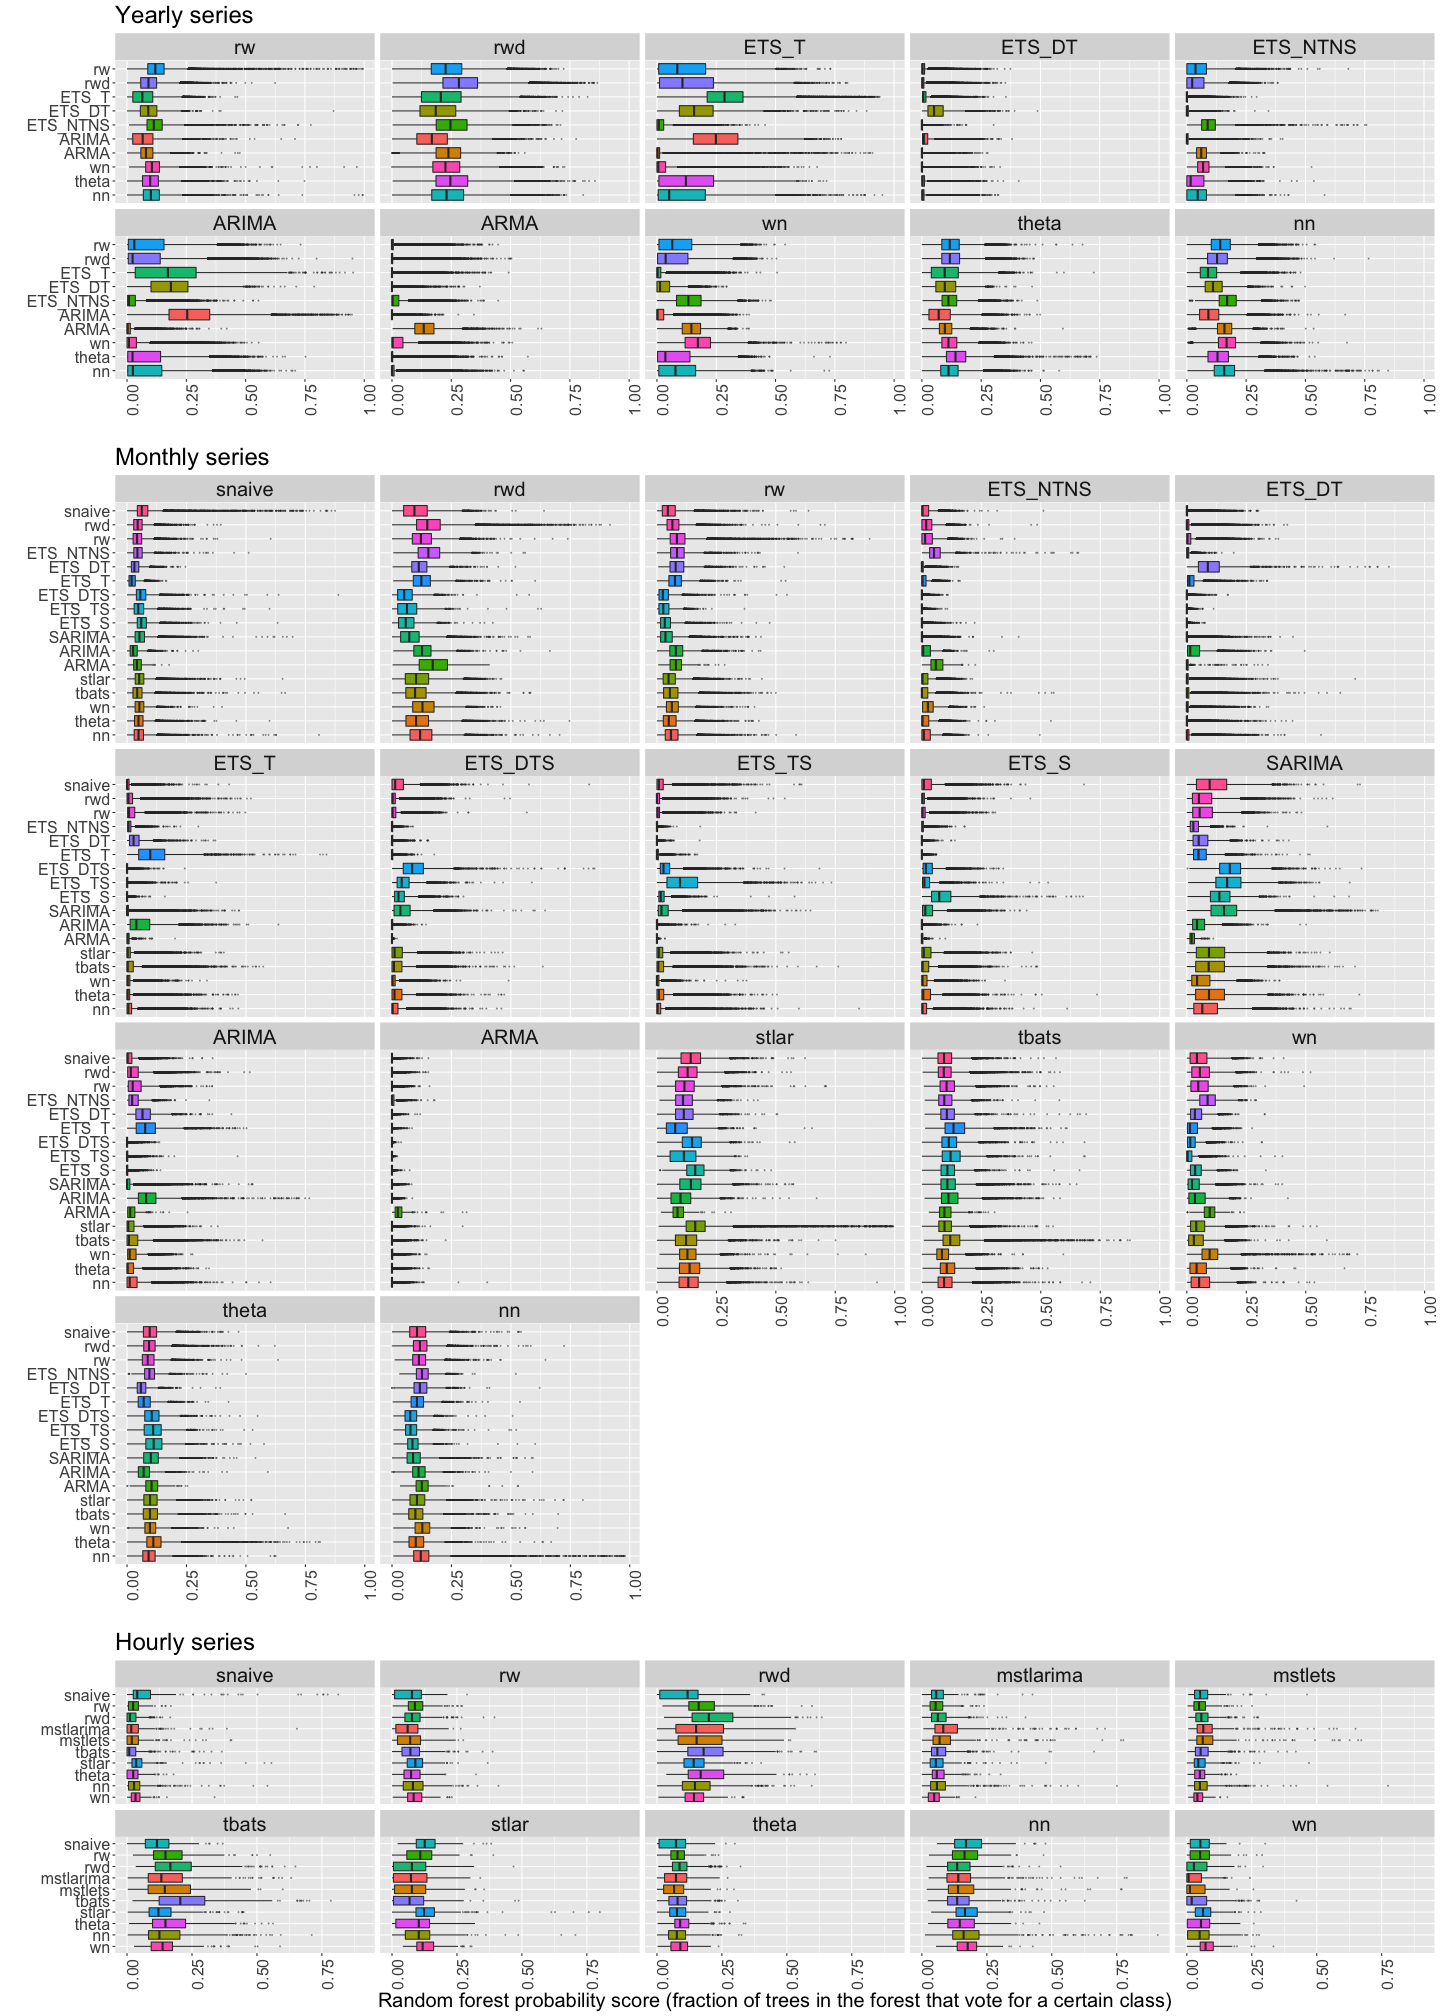
\includegraphics[width=\textwidth]{figure/yearlyoob-1} 

}

\caption{Visualisation of the vote matrix for yearly, monthly and hourly series. Each panel shows the forecast models considered as classlabels. The X-axis denotes the fraction of trees in the forest that vote for the classlabel in the panel name. The Y-axis corresponds to class label of the best forecast model identified based on MASE and sMAPE. On each row, distribution of correctly classified class dominates, indicating a good classification of the meta-learner.}\label{fig:yearlyoob}
\end{figure}

\clearpage

\hypertarget{which-features-are-the-most-important-and-where-are-they-important}{%
\subsection{Which features are the most important and where are they important?}\label{which-features-are-the-most-important-and-where-are-they-important}}

\begin{figure}[h]

{\centering 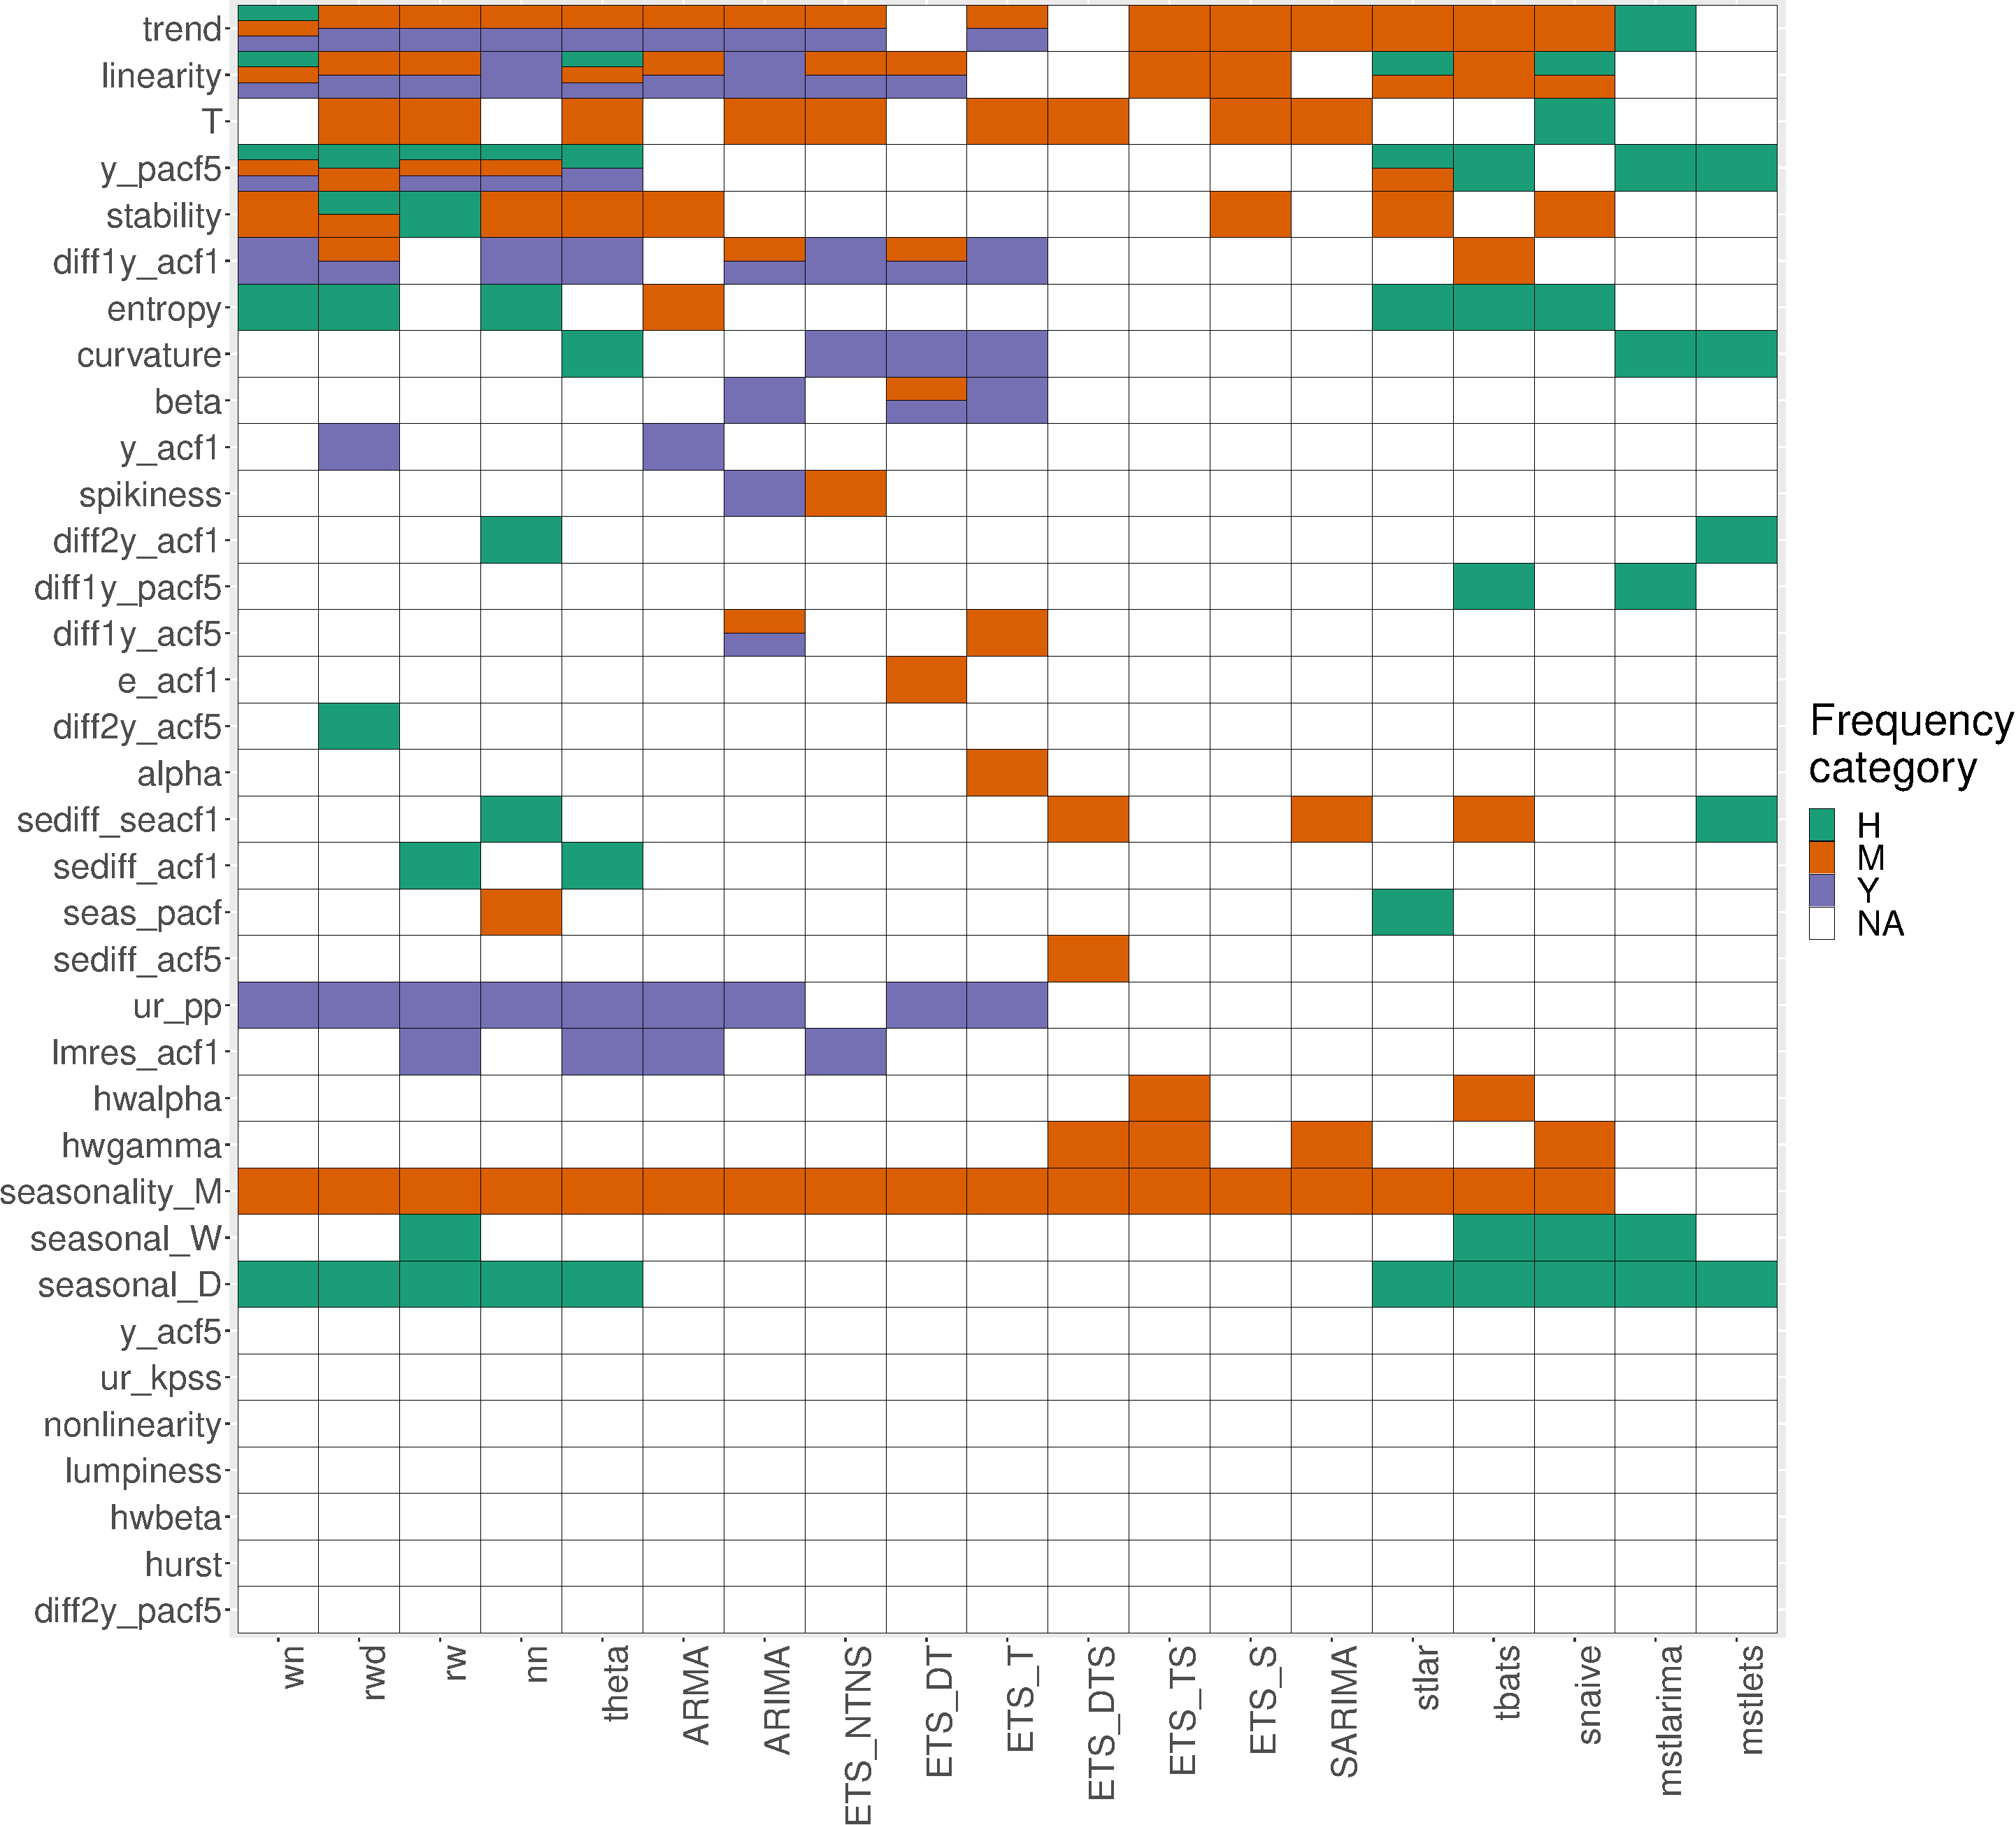
\includegraphics[width=\textwidth]{figure/viplot-1} 

}

\caption{Visualisation  of top five features across frequency categories and classes. The X-axis denotes the features and Y-axis denotes the forecast model classes. The cell colours denote the frequency group in which the fetures ranked among top five. The feature importance is evaluated based on the three measures: i) permutation-based VI, ii) PD-based VI measure, and iii) ICE-based VI measure. Strength of trend, linearity and strength of seasonality have been selected among top five features across many classes.}\label{fig:viplot}
\end{figure}

\autoref{fig:viplot} shows top-5 most important features the within each class across yearly, monthly and daily series. The main point here is strength of trend, sum of first five partial autocorrelation coefficients, stability, the first ACF value of the differenced series and linearity are the most important features across many classes and frequency categories. The information about the strength of trend in the series, linearity and sum of first five partial autocorrelation are very important when selecting white noice process among all frequency categories. For yearly data, the test statistic based on the Phillips-Perron unit root test has been ranked among top-5 within all classes. In addition to linearity, the other features related to different types of trend (damped trend, measured by beta, and exponential trend, measured by curvature) are assigned a very high importance within ETS\_T, ETS\_DT and ETS\_NTNS, which handle different versions of trend within the ETS family. The length of time series (T) and stability are assigned a very high importance within monthly series. For seasonal time series strength of seasonality has been selected among top-5 features across all classes. For hourly data, the strength of daily seasonality (measured by seasonal\_d) appears to be more important than the strength of weekly seasonality (measured by seasonal\_w). In addition to the strength of seasonality, the other features such as ACF, PACF-based features related to seasonal lag and seasonally differenced series are also ranked among top five within some classes.

\hypertarget{when-and-how-are-features-linked-to-the-prediction-outcome}{%
\subsection{When and how are features linked to the prediction outcome?}\label{when-and-how-are-features-linked-to-the-prediction-outcome}}

\autoref{fig:pdpyearlyurpp} shows the partial dependency curves of the of the Phillips-Perron test statistic.
Within each class the displayed relationship is consistent with the theoretical expectations. For example, a high negative value of the Phillips-Perron test statistic indicates a stationarity of the series, while a positive value of the test statistic indicates nonstationarity of the series. According to \autoref{fig:pdpyearlyurpp}, we can see that the probability of selecting an ETS model with a trend component and ARIMA models increases steadily as ur\_pp increases, while the opposite relationship could be observed for ARMA and WN.

For monthly series, the strength of seasonality is the most important features across all classes. According to \autoref{fig:pdpmonthlyseasonality}, it is immediately apparent that the probability of selecting a seasonal forecast model increases as the strength of seasonality increases. The length of time series is also assigned a high importance within many classes. Partial dependency curves of \autoref{fig:pdpmonthlyT} reveal longer time series tend to select highly parameterised models or models involving seasonal components such as (ETS\_TS, ETS\_DTS, ETS\_S, SARIMA, tbats), while shorter series tend to select simple models such as random walk, random walk with drift etc.

The partial dependency plots of the strength of seasonalities for hourly series are shown in \autoref{fig:seasonalityhourly}. According to \autoref{fig:seasonalityhourly}, the probability of selecting random walk, random walk with drift, theta and white noise process decreases with a higher value of strength of daily seasonality. On the other hand, the probability of the selecting random walk model increases as the strength of weekly seasonality increases. The partial dependency plots of entropy are shown in \autoref{fig:entropyhourly}. The entropy measures forecastability of time series. We can see that the probability of selecting random walk with drift and tbats decreases as the entropy increases. This is consistent with our theoretical expectations. In other words, if the series has a clear trend or a clear trigonometric pattern, the forecastability of the time series is high and the entropy is low. For highly trended series the random walk with drift model is suitable, while for a series with trigonometric pattern the tbats model is suitable. The curvature of the series is appeared among top-5 within mstlarim, mstlets and theta classes for hourly series. According to the \autoref{fig:curvaturehourly}, probability of selecting these models show a non-monotonic relationship with the curvature.

\autoref{fig:pdpmonthlyhourlyStability} show the partial dependency plot of stability. One notable difference between the yearly series and monthly series is that for monthly series, the feature stability is ranked among the top five within many classes. The feature stability does not appear to be ranked among the top 5 within any of the classes for yearly series. The stability is ranked important only within random walk and random walk with drift for hourly series. According to the \autoref{fig:pdpmonthlyhourlyStability} we can see that the probability of selecting white noise models increases as stability increases for monthly series while for hourly series the probability of selecting random walk models and random walk with drift models increases as stability increases. The feature diff1y\_acf1 is useful in determining the difference stationarity of the time series. This feature has been ranked among the top-five within the classes of yearly and monthly series. The associated partial dependency plots are shown in \autoref{fig:diff1yacf1}. It is interesting to observe that difference stationary series are less likely to select ARIMA models. The reason could be difference stationary series are more likely to select random walk models, and ETS models. Furthermore, partial difference curve corresponds to white noise class shows difference stationary series have high chance of selecting white noise modesl. This unusal pattern could be due to over-differencing of the series or interaction effect between features.

The features, sum of the first five partial autocorrelation coefficients, strength of trend and linearity are the most commonly selected features within many classes across all three frequency category. The partial dependency plot for the sum of the first five partial autocorrelation coefficients are shown in \autoref{fig:ypacf5}. All curves shows a turning point in the relations around 1. It also appears that the pattern of the relationship varies across classes as well as frequency categories. \autoref{fig:pdpyearlytrend} show the partial dependency curves for strength of trend. The probability of selecting an ETS model without trend components: ETS (N,N,N), white noise process and ARMA is extremely low when the strength of trend is extremely high, while the opposite relationship can be observed for other classes. The partial dependency plot for linearity is shown in \autoref{fig:linearity}. According to \autoref{fig:linearity} for yearly series random walk with drift and ARMA classes are highly sensitive to the value of linearity around 0. However, the partial dependency curves of linearity for other combinations are relatively flat throughout the range. This could be due to the interaction effect of linearity with other features.

\begin{figure}[h]

{\centering 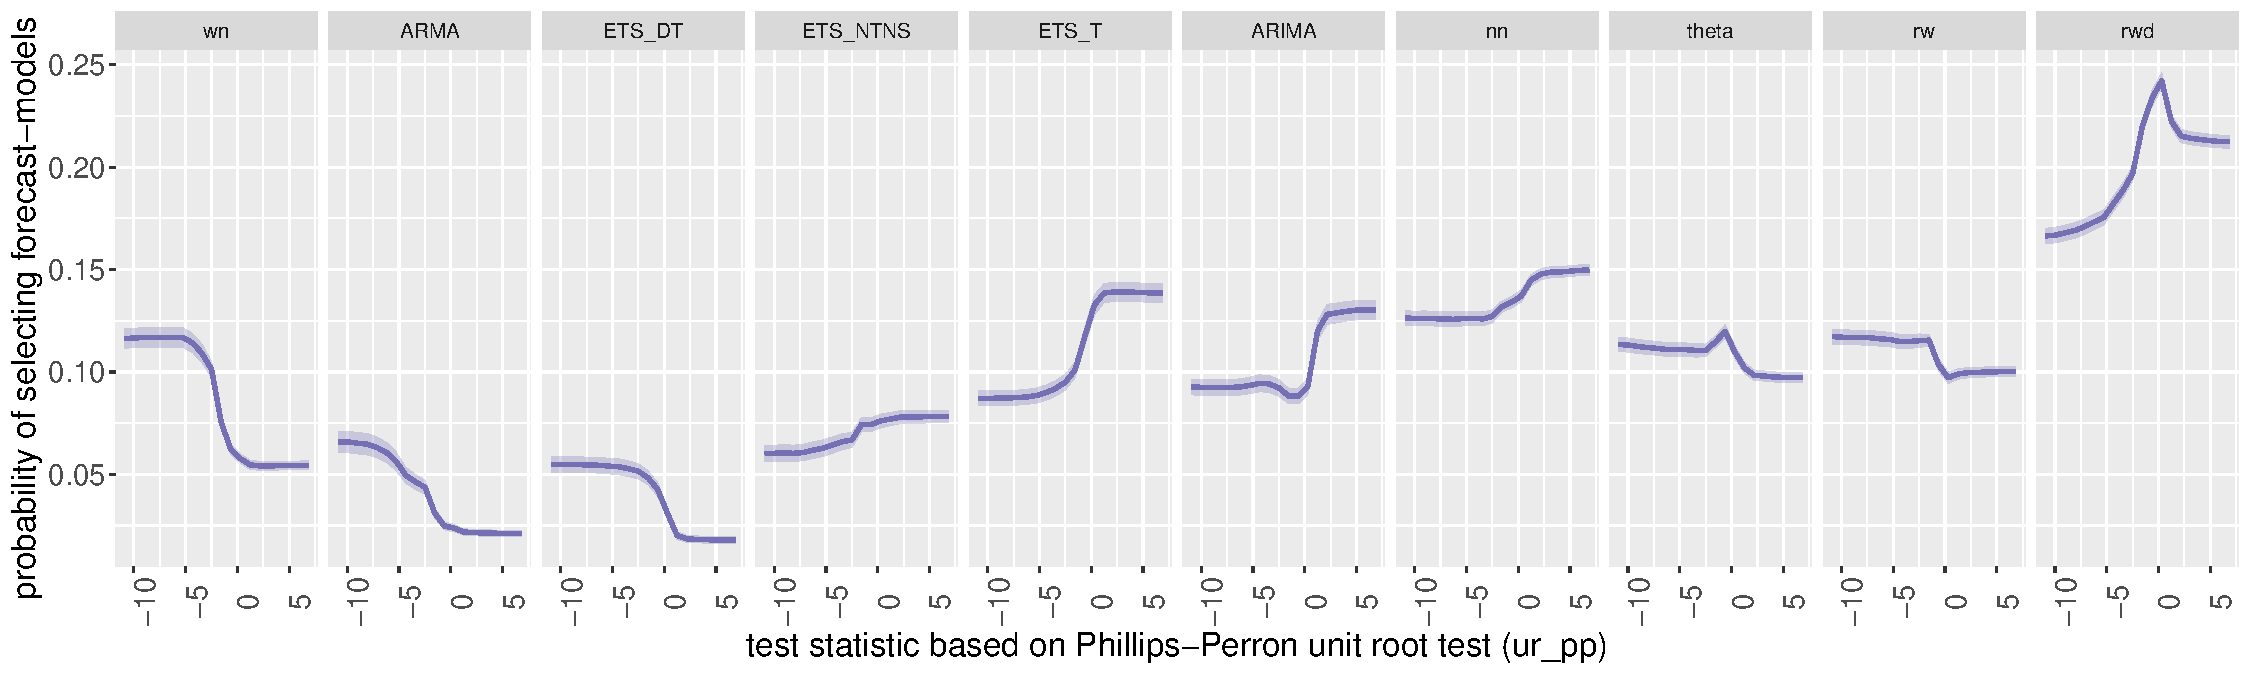
\includegraphics[width=\textwidth]{figure/pdpyearlyurpp-1} 

}

\caption{Partial dependence plots for Phillips-Perrorn unit root test statistic. The shading shows the 95\% confidence intervals. Y-axis denotes the probability of belonging to the corresponding class. All classes show a turning point in the relationship around zero.}\label{fig:pdpyearlyurpp}
\end{figure}

\begin{figure}[h]

{\centering 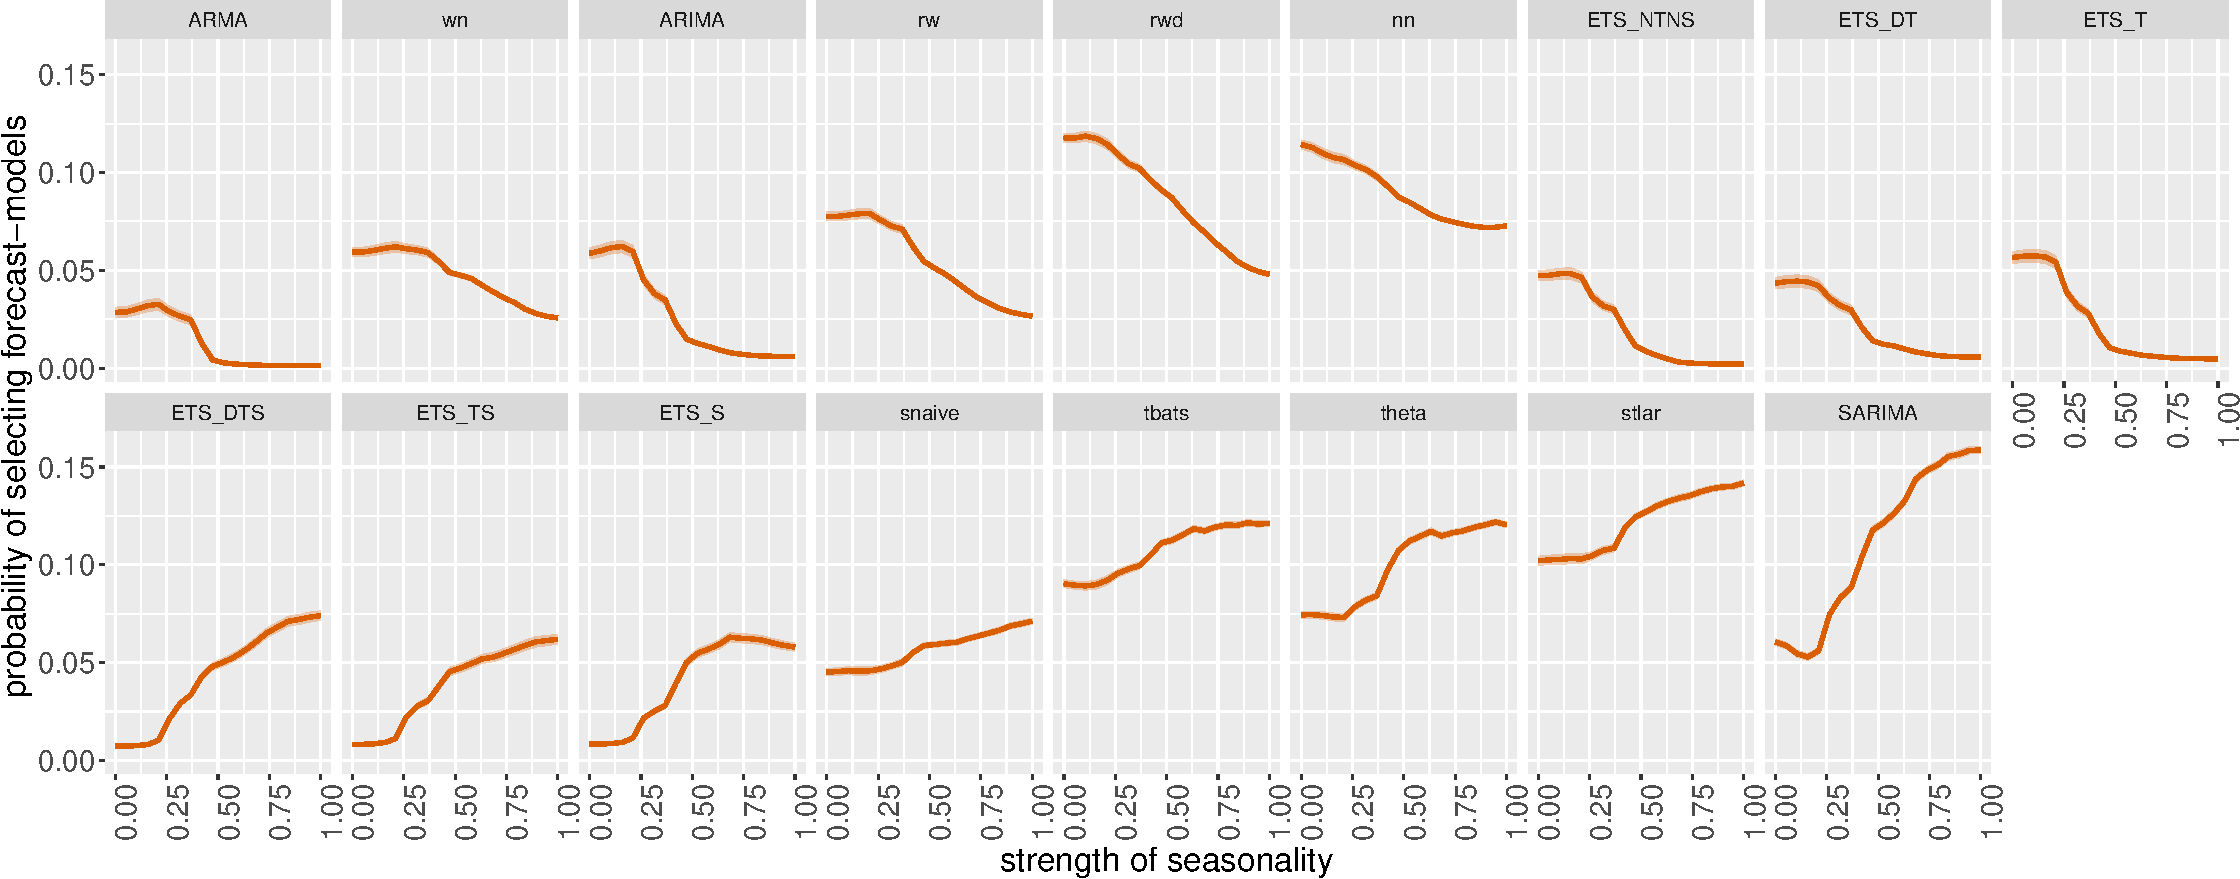
\includegraphics[width=\textwidth]{figure/pdpmonthlyseasonality-1} 

}

\caption{Partial dependence plots for strength of seasonality for monthly series. The shading shows the 95\% confidence intervals. Y-axis denotes the probability of belonging to the corresponding class. Probability of selecting forecast models with seasonal components increases as seasonality increases.}\label{fig:pdpmonthlyseasonality}
\end{figure}

\begin{figure}[h]

{\centering 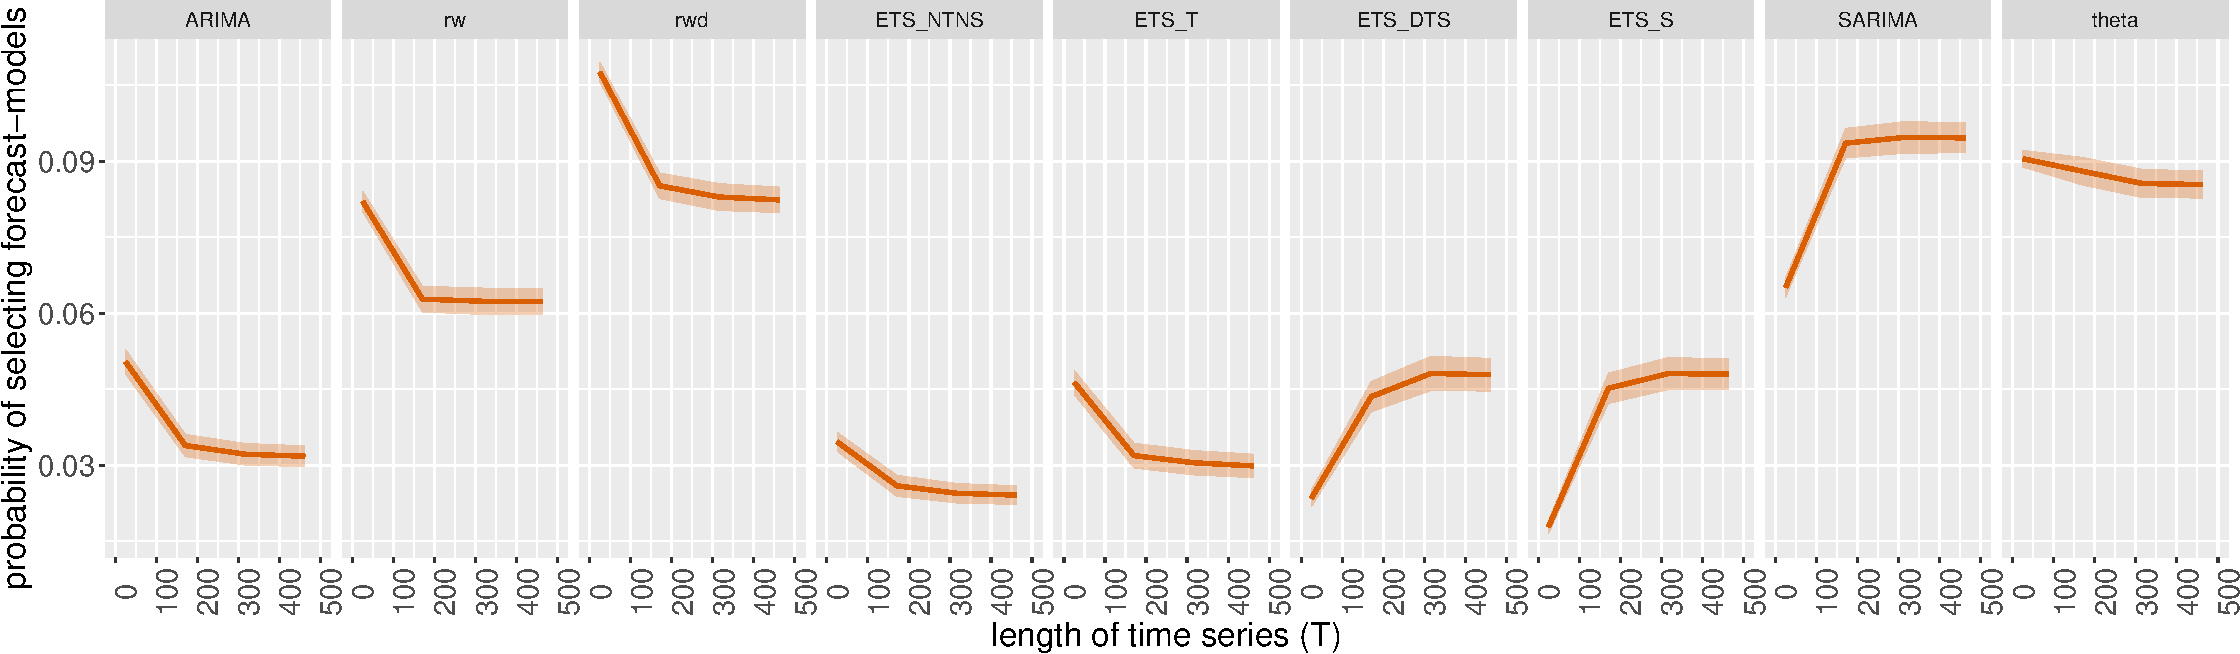
\includegraphics[width=\textwidth]{figure/pdpmonthlyT-1} 

}

\caption{Partial dependence plots for length of time series (T). The shading shows the 95\% confidence intervals. Y-axis denotes the probability of belonging to the corresponding class. Probability of selecting rw and rwd decreases as the length > 500.}\label{fig:pdpmonthlyT}
\end{figure}

\begin{figure}[h]

{\centering 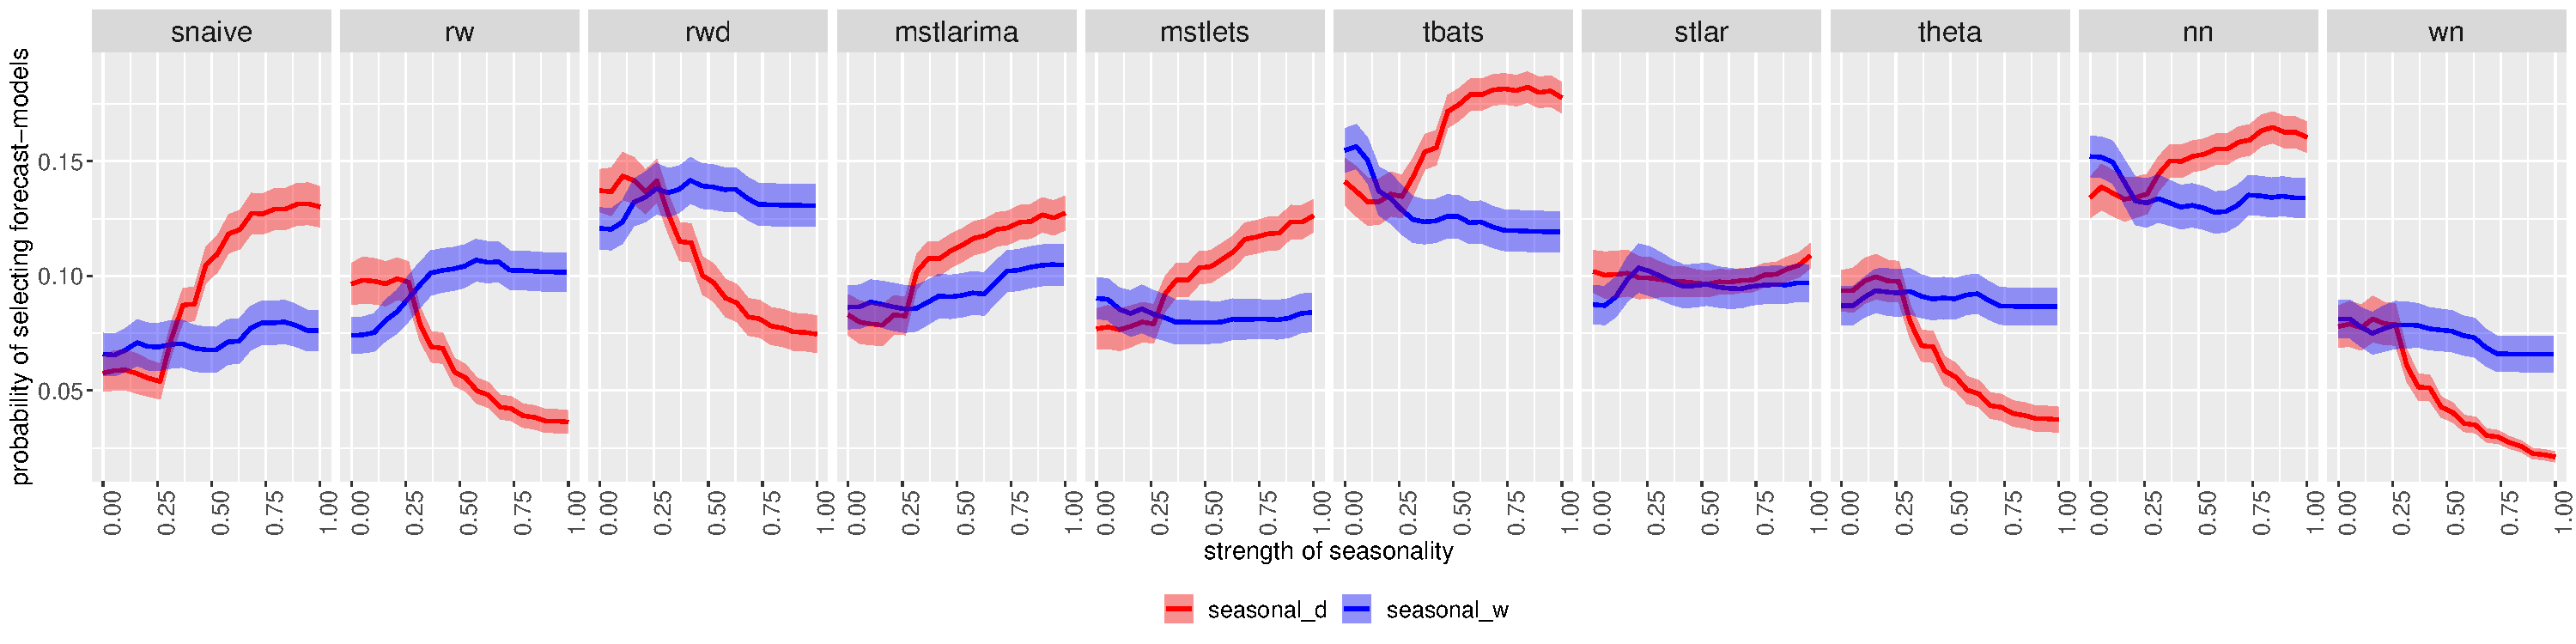
\includegraphics[width=\textwidth]{figure/seasonalityhourly-1} 

}

\caption{Partial dependence plots for strength of seasonality for hourly series. The shading shows the 95\% confidence intervals. Y-axis denotes the probability of belonging to the corresponding class.}\label{fig:seasonalityhourly}
\end{figure}

\begin{figure}[h]

{\centering 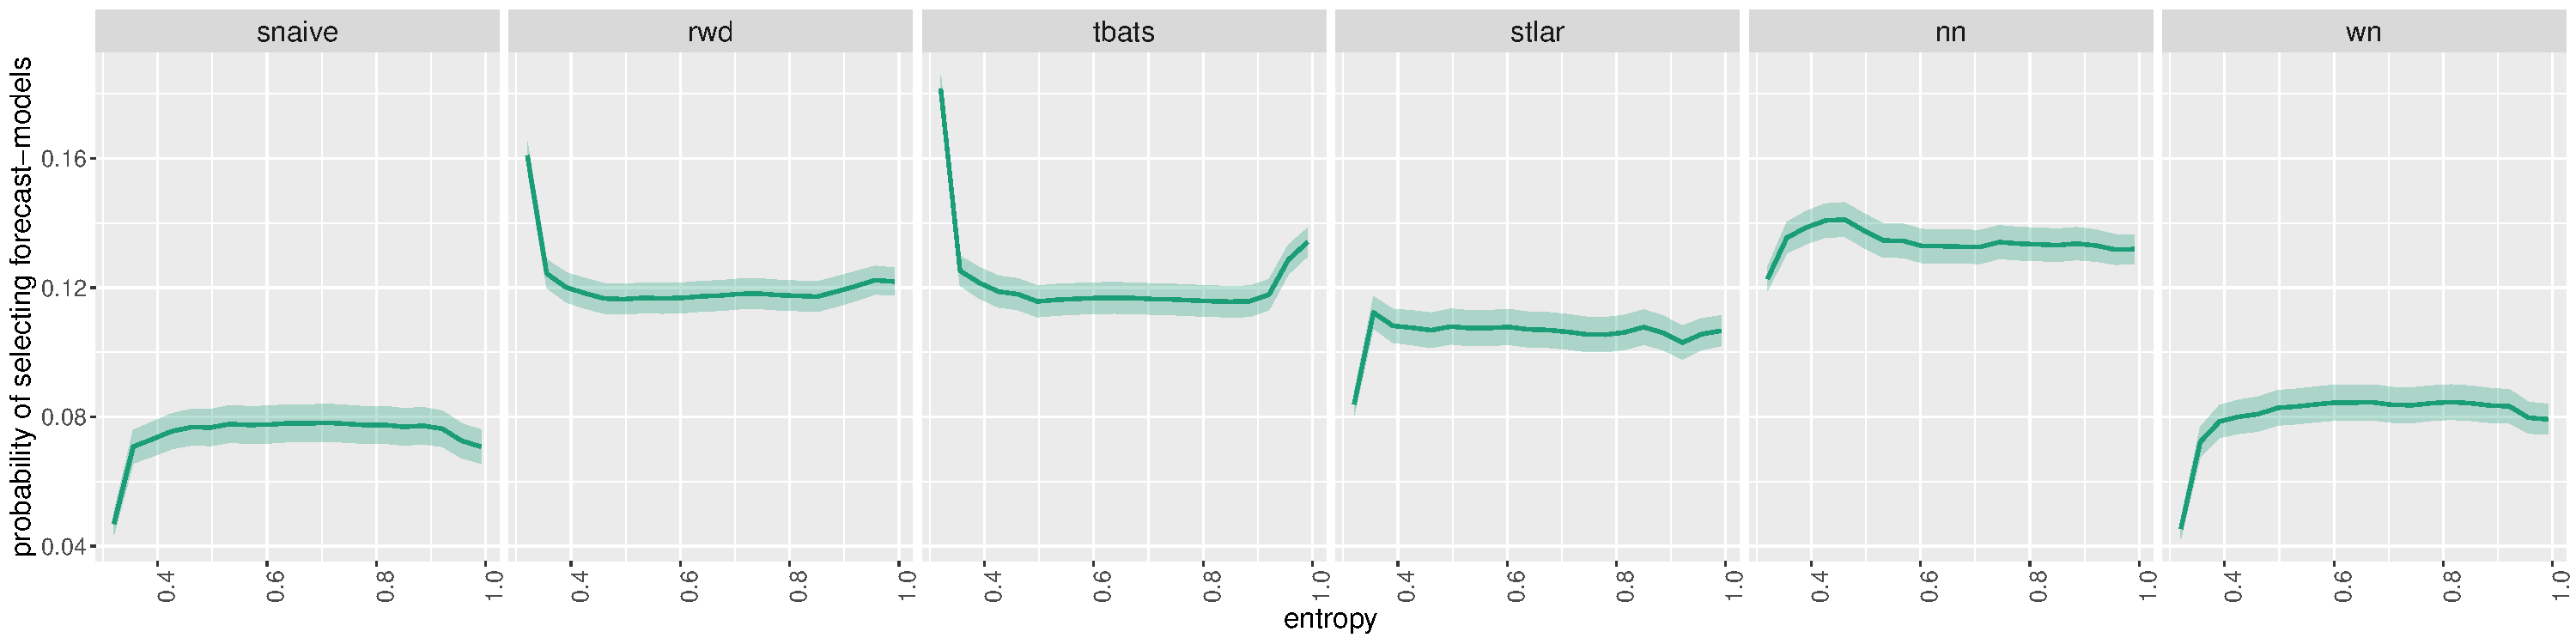
\includegraphics[width=\textwidth]{figure/entropyhourly-1} 

}

\caption{Partial dependence plots for entropy for hourly series. The shading shows the 95\% confidence intervals. Y-axis denotes the probability of belonging to the corresponding class.}\label{fig:entropyhourly}
\end{figure}

\begin{figure}[h]

{\centering 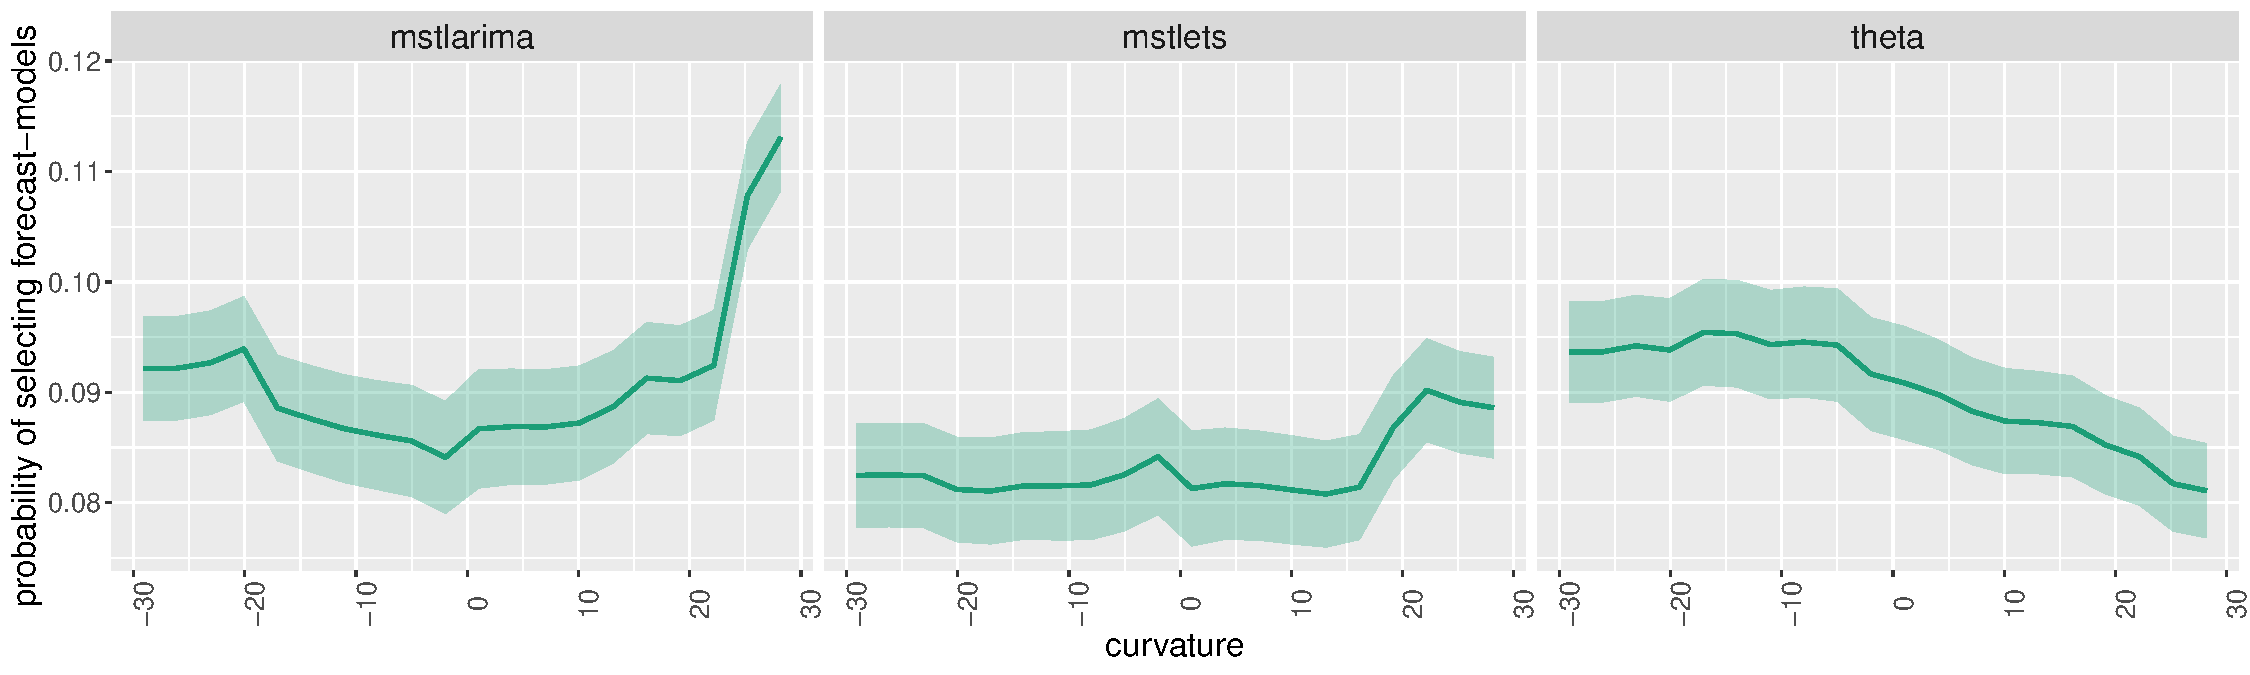
\includegraphics[width=\textwidth]{figure/curvaturehourly-1} 

}

\caption{Partial dependence plots for curvature for hourly series. The shading shows the 95\% confidence intervals. Y-axis denotes the probability of belonging to the corresponding class.}\label{fig:curvaturehourly}
\end{figure}

\begin{figure}[h]

{\centering 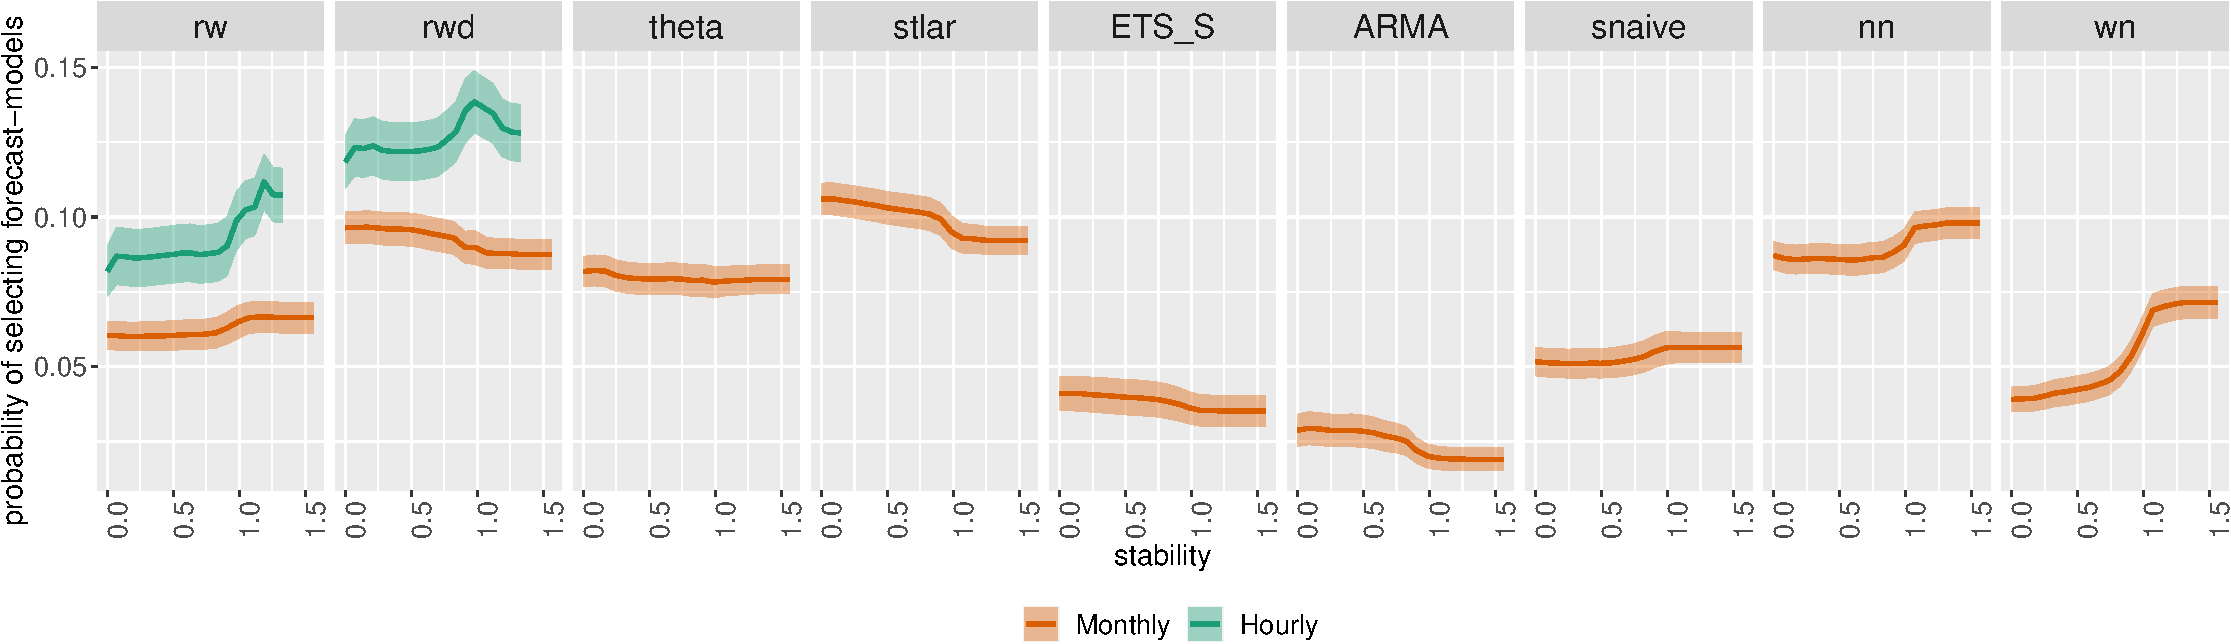
\includegraphics[width=\textwidth]{figure/pdpmonthlyhourlyStability-1} 

}

\caption{Partial dependence plots for stability for monthly and hourly series. The shading shows the 95\% confidence intervals. Y-axis denotes the probability of belonging to the corresponding class.}\label{fig:pdpmonthlyhourlyStability}
\end{figure}

\begin{figure}[h]

{\centering 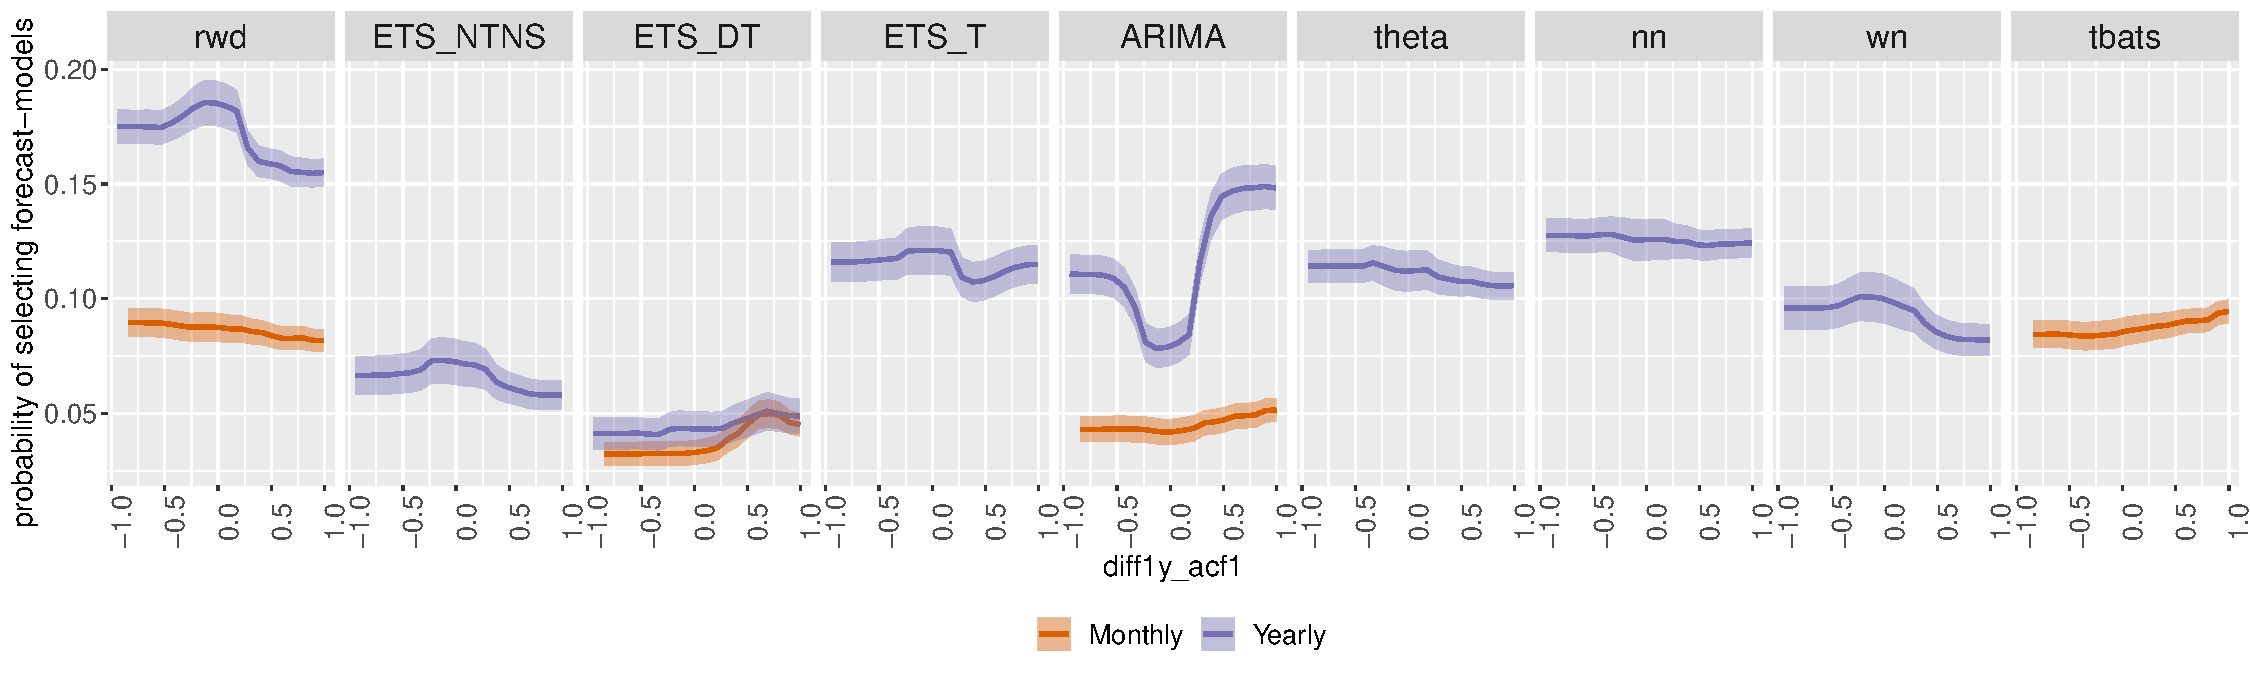
\includegraphics[width=\textwidth]{figure/diff1yacf1-1} 

}

\caption{Partial dependence plots for diff1y\_acf1 for yearly and monthly series. The shading shows the 95\% confidence intervals. Y-axis denotes the probability of belonging to the corresponding class.}\label{fig:diff1yacf1}
\end{figure}

\begin{figure}[h]

{\centering 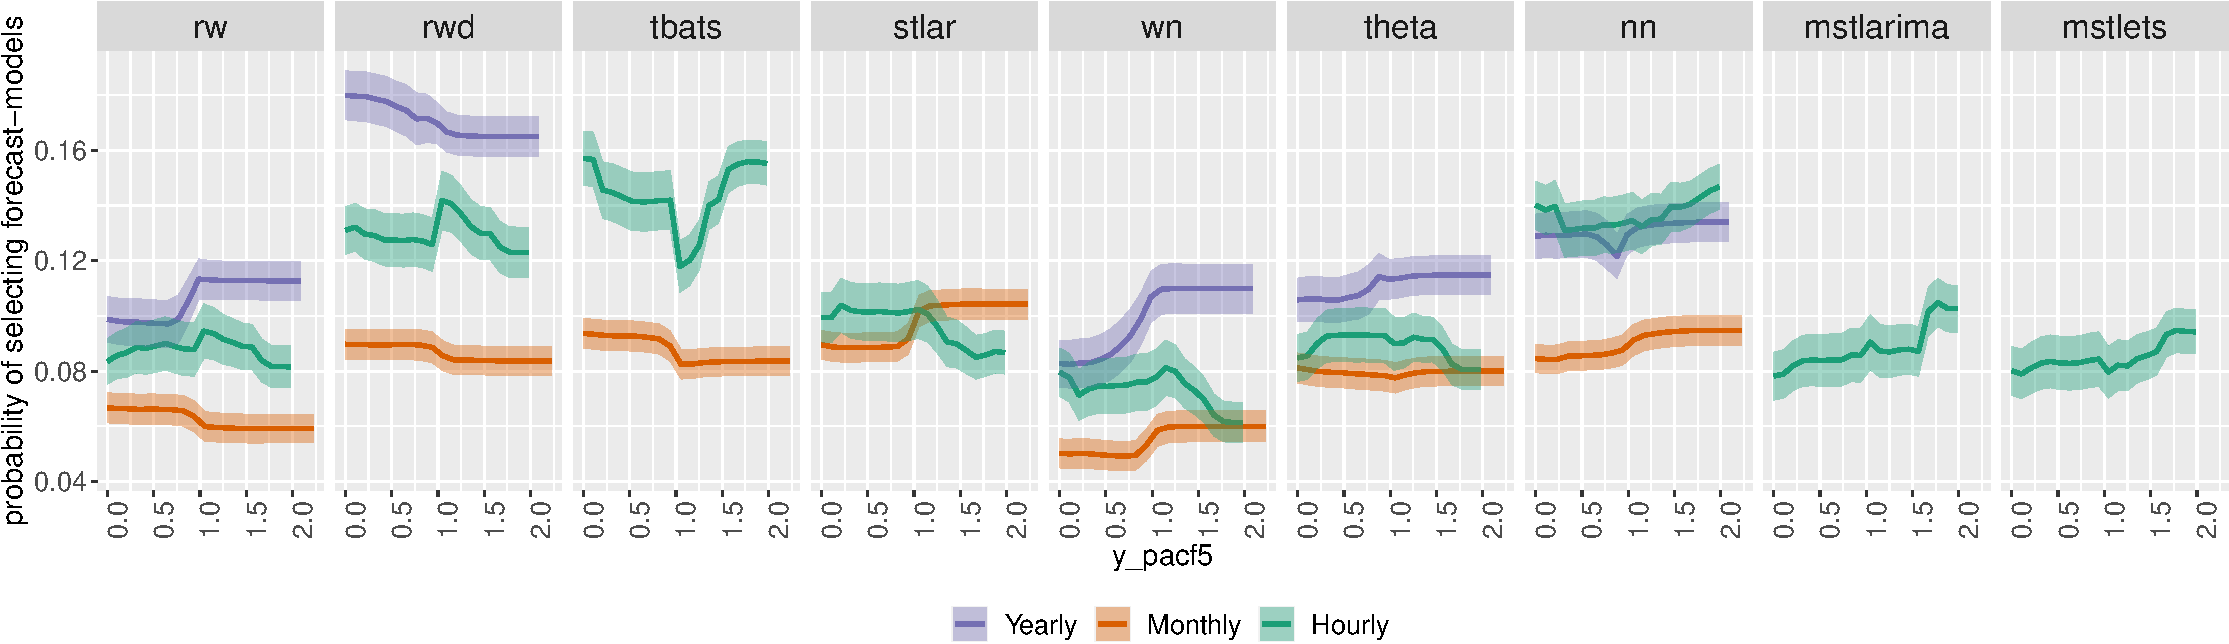
\includegraphics[width=\textwidth]{figure/ypacf5-1} 

}

\caption{Partial dependence plots for y\_pacf5 for yearly monthly and hourly series. The shading shows the 95\% confidence intervals. Y-axis denotes the probability of belonging to the corresponding class. }\label{fig:ypacf5}
\end{figure}

\begin{figure}[h]

{\centering 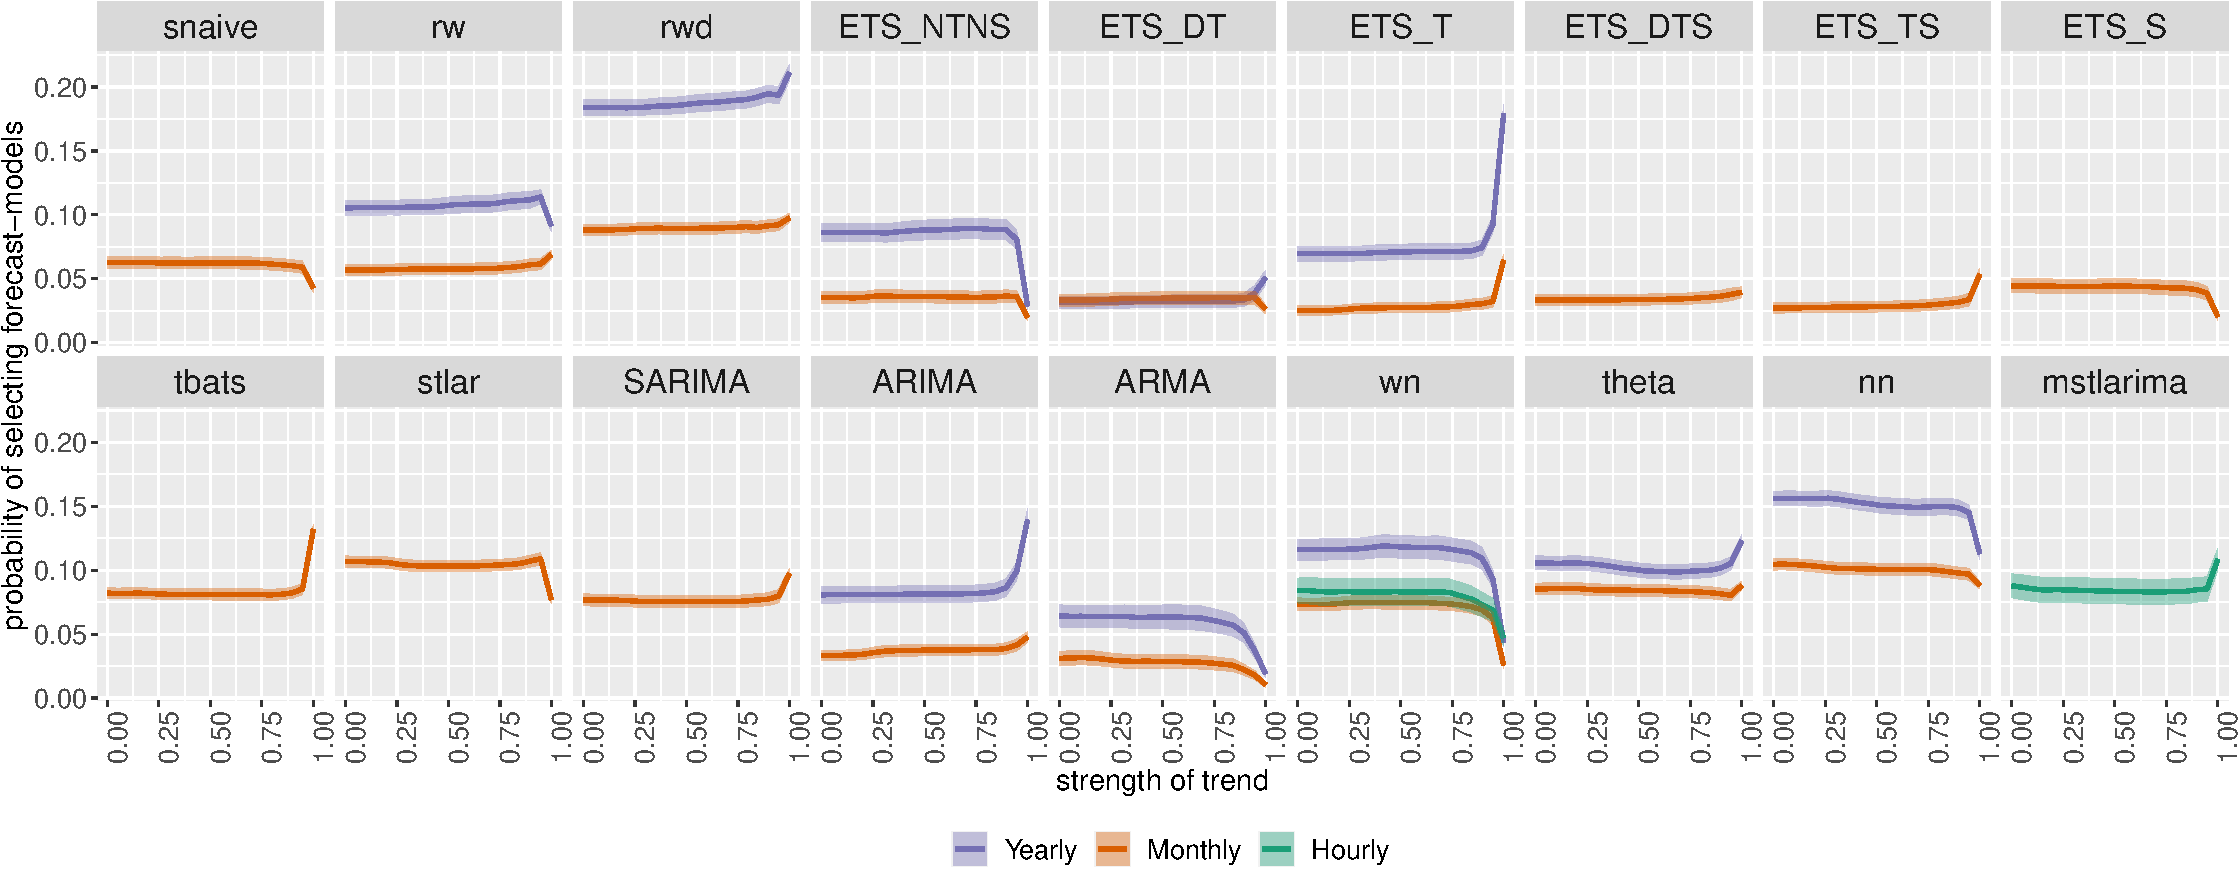
\includegraphics[width=\textwidth]{figure/pdpyearlytrend-1} 

}

\caption{Partial dependence plots for trend for yearly and monthly series. The shading shows the 95\% confidence intervals. Y-axis denotes the probability of belonging to the corresponding class. Probability of selecting ETS models without a trend component and stationary models (WN and ARMA) decreases for an extremely high value of trend.}\label{fig:pdpyearlytrend}
\end{figure}

\clearpage

\begin{figure}[h]

{\centering 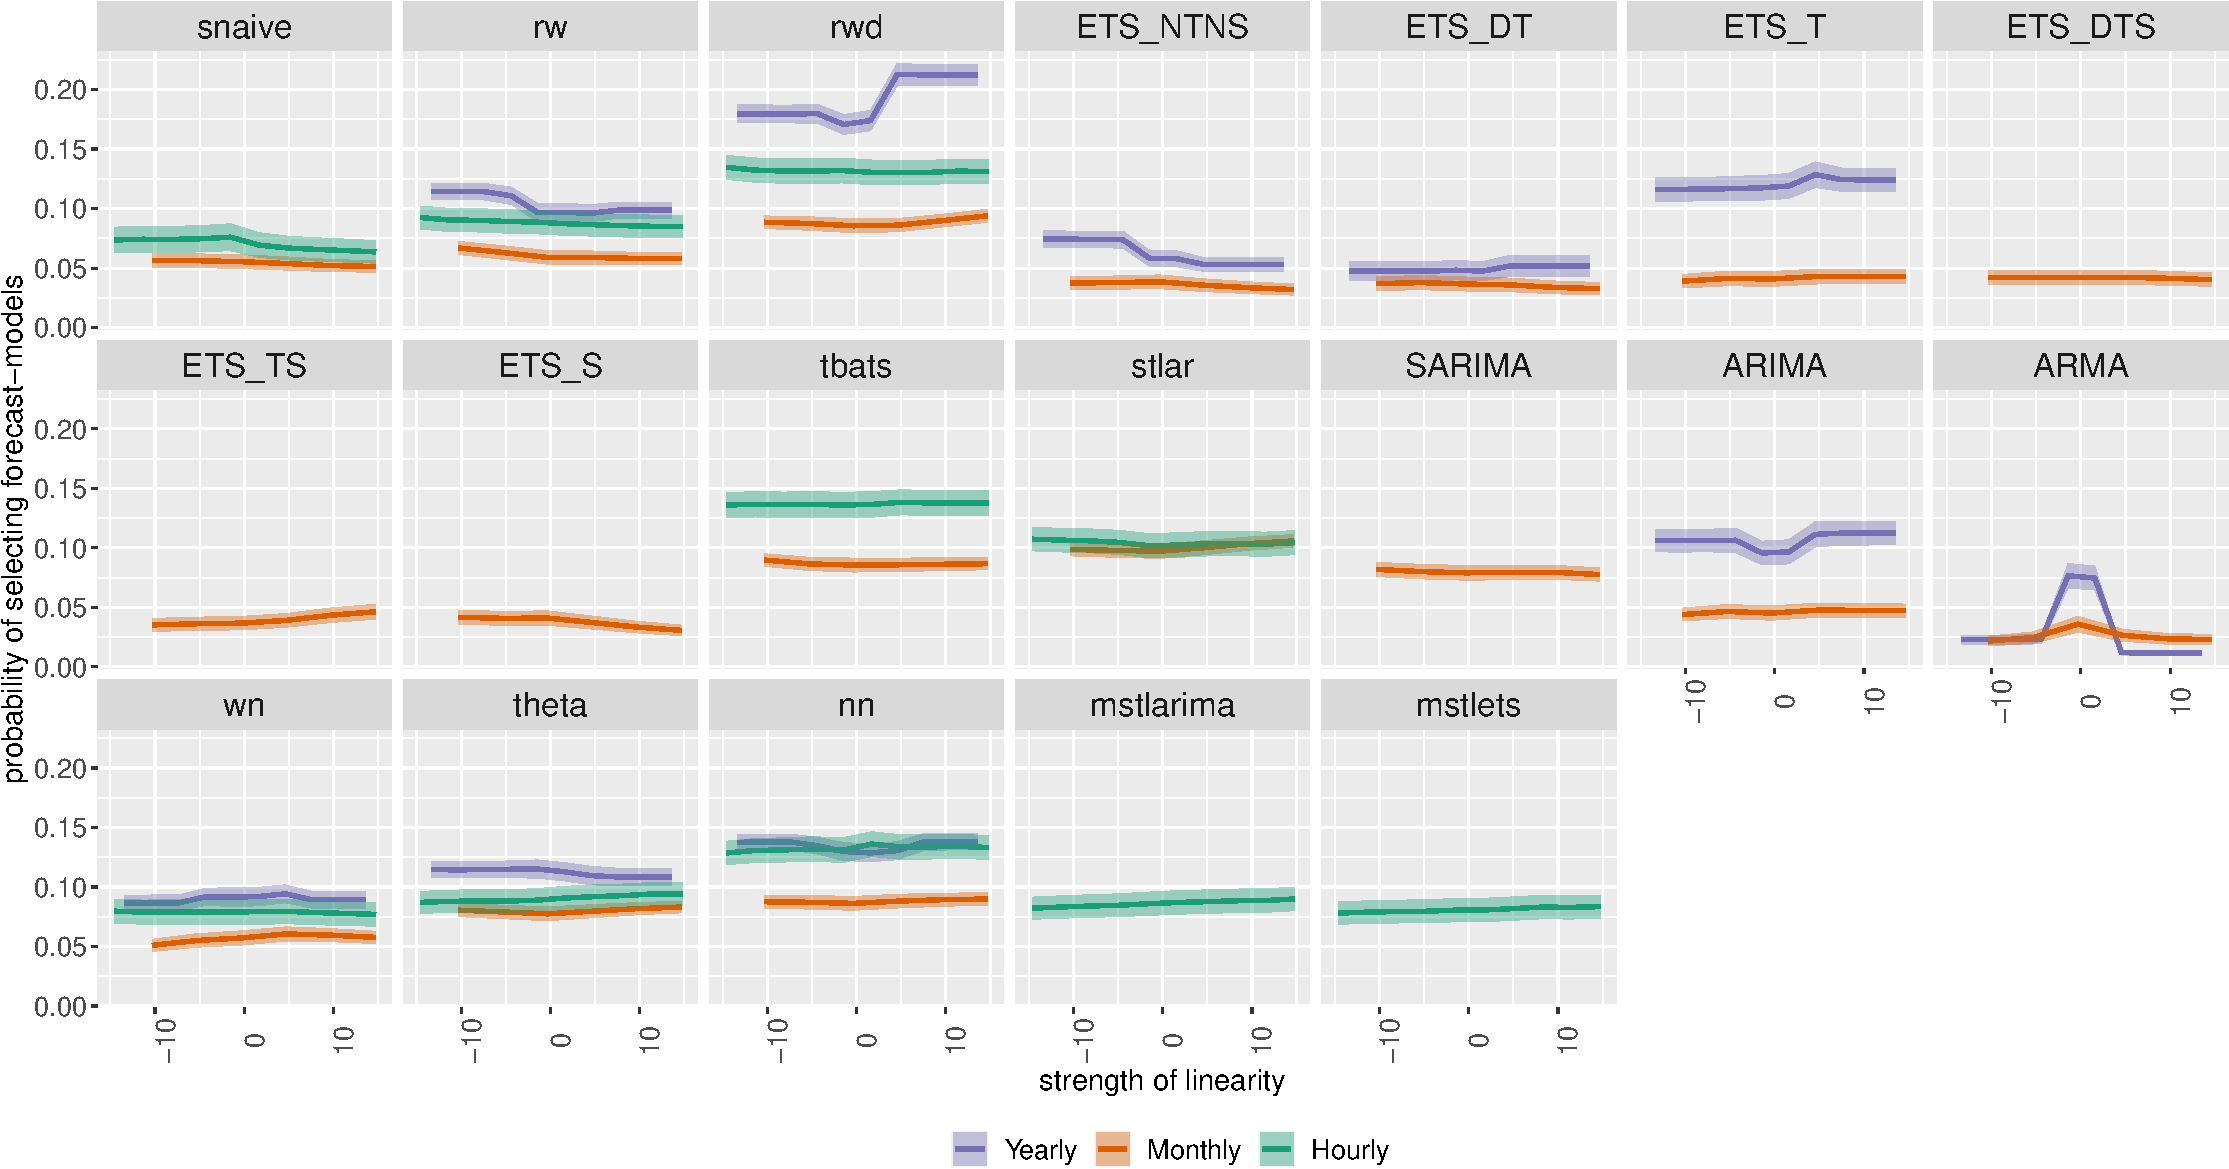
\includegraphics[width=\textwidth]{figure/linearity-1} 

}

\caption{Partial dependence plots for linearity for yearly monthly and hourly series. The shading shows the 95\% confidence intervals. Y-axis denotes the probability of belonging to the corresponding class. }\label{fig:linearity}
\end{figure}

\begin{figure}[h]

{\centering 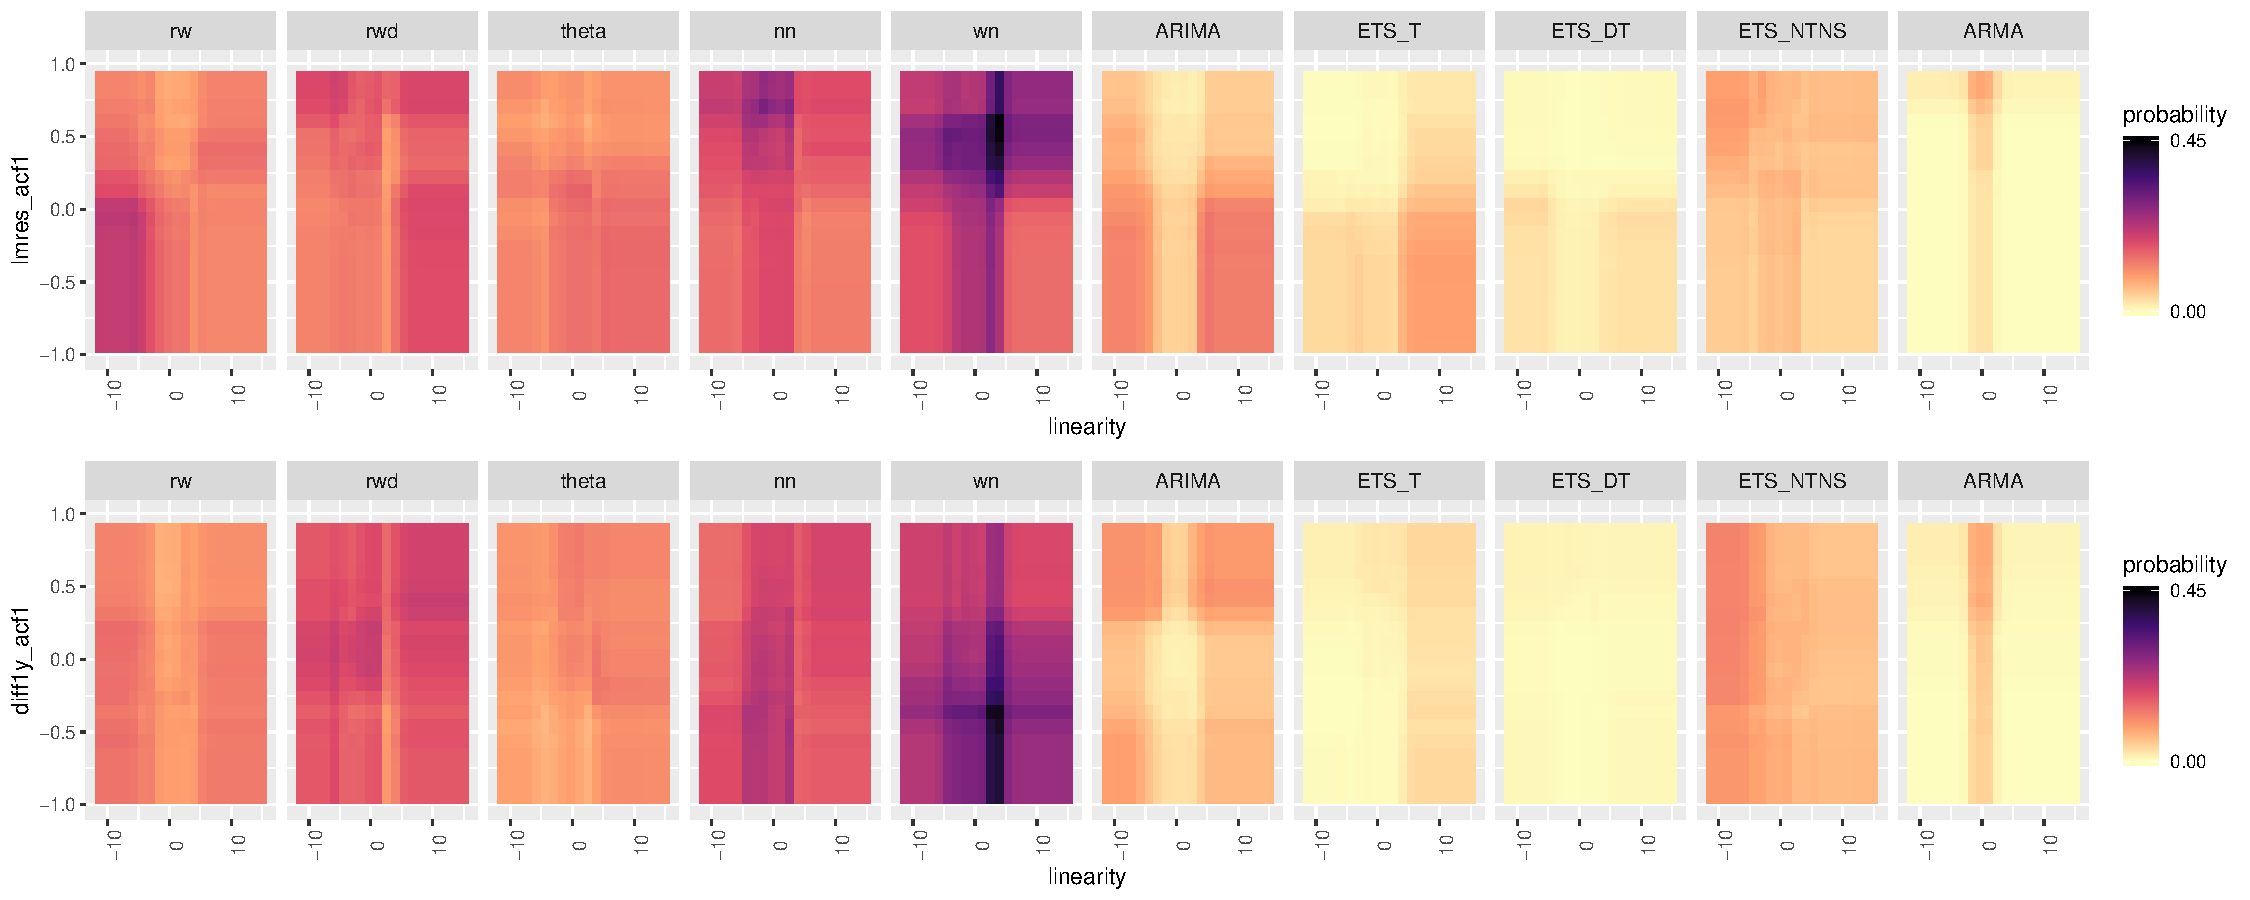
\includegraphics[width=\textwidth]{figure/y2dpdp-1} 

}

\caption{Two-way partial dependence plots for linearity for yearly series. Dark regions show the high probability of belonging to the corresponding class shown in the plot title.}\label{fig:y2dpdp}
\end{figure}

The two-way partial dependency plots of linearity are explored to see how linearity behaved in the presence of other top-5 features. The associated two-way partial dependency plots are shown in \autoref{fig:y2dpdp}, \autoref{fig:m2dpdp} and \autoref{fig:h2dpdp} for yearly, monthly and hourly series respectively. According to the \autoref{fig:y2dpdp} within wn, random walk, theta and nn classes linearity shows a pattern of interactivity with lmres\_acf1 and diff1y\_acf1. Within both ARIMA and ARMA classes main effect of linearity dominates. This is consistent with partial dependency curves we observed in \autoref{fig:linearity}. For monthly series, linearity shows interactivity with acf value at the first seasonal lag of seasonally-differenced series, stability, first ACF value at the remainder series and a parameter estimate of ETS(A, A, A) model. According to \autoref{fig:m2dpdp}, we can see there is a unique pattern of interactivity existing within each class. The two-way partial dependency plot for hourly series between the ACF value at the first seasonal lag of seasonally-differenced series and linearity are shown in \autoref{fig:h2dpdp}. The inconsistent level of colour intensity throughout the panels in tbats, nn and stlar indicate probability of selecting the corresponding forecast models changes according to the changes in both the features. Within rw and mstlarima we can see a separation between the lower half and the upper half due to the main effect of sediff\_seacf1. The partial dependency curves of theta for stability is relatively flat. \autoref{fig:thetapdp} shows how trend, length, first autocorrelation coefficient of the differenced series interact with stability within different ranges. For example, \autoref{fig:thetapdp} as length of time series decreases, a pattern of interaction is visible with stability.

\begin{figure}[h]

{\centering 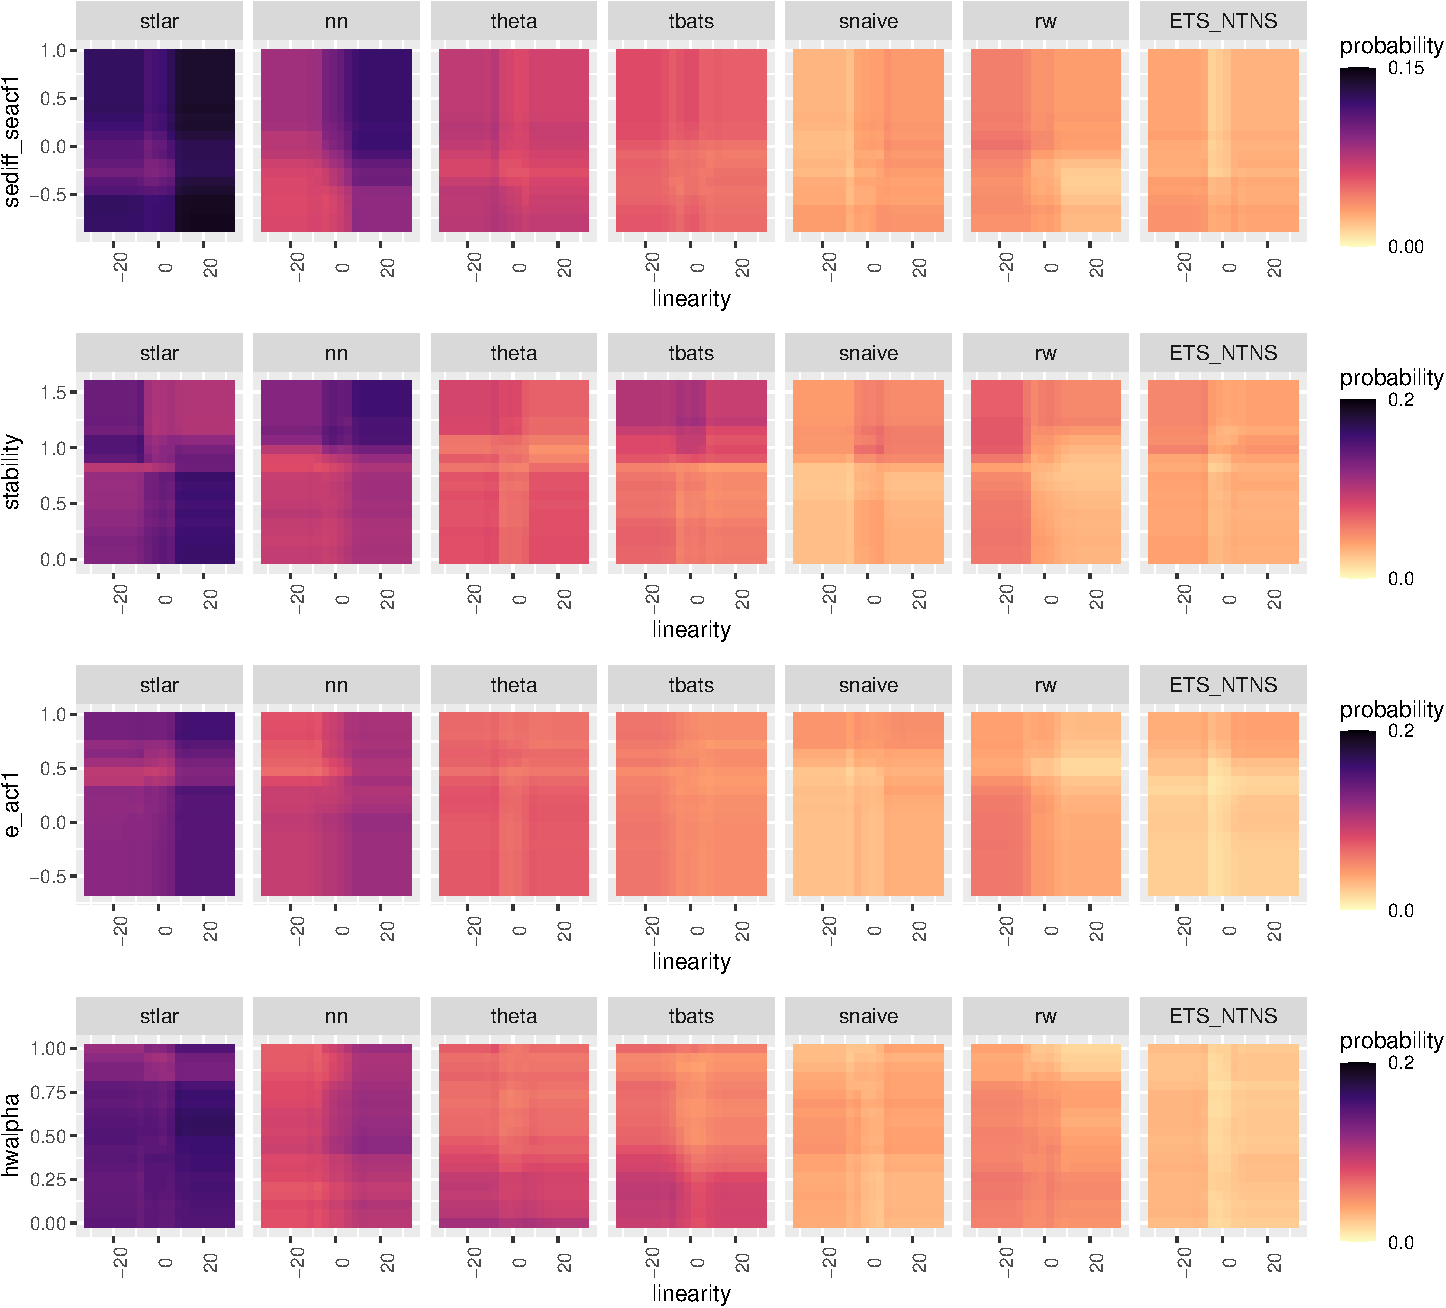
\includegraphics[width=\textwidth]{figure/m2dpdp-1} 

}

\caption{Two-way partial dependence plots for linearity for monthly series. Dark regions show the high probability of belonging to the corresponding class shown in the plot title.}\label{fig:m2dpdp}
\end{figure}

\clearpage

\begin{figure}[h]

{\centering 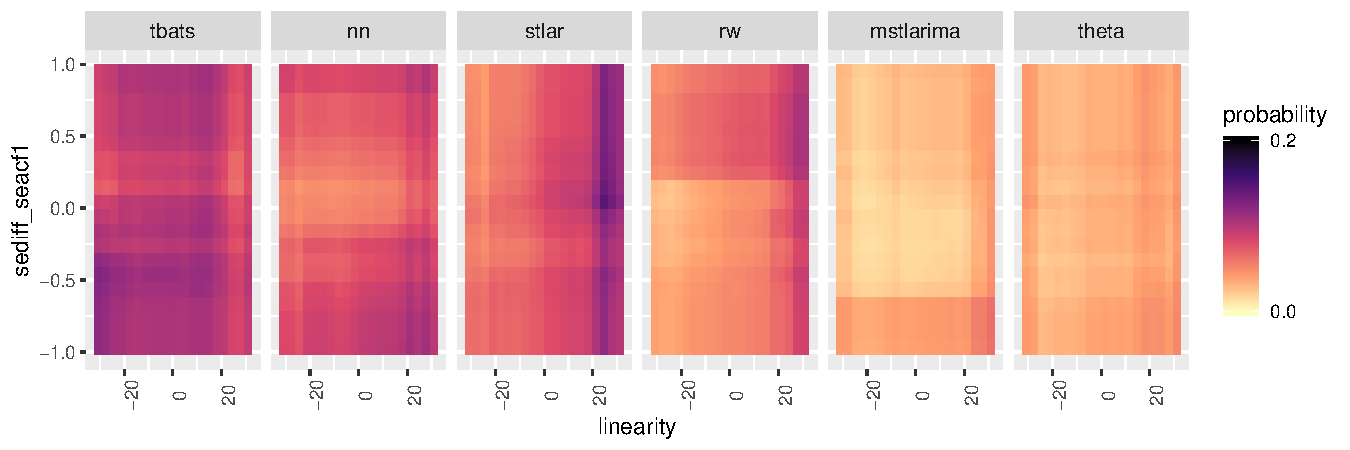
\includegraphics[width=\textwidth]{figure/h2dpdp-1} 

}

\caption{Two-way partial dependence plots for linearity for hourly series. Dark regions show the high probability of belonging to the corresponding class shown in the plot title.}\label{fig:h2dpdp}
\end{figure}

\begin{figure}[h]

{\centering 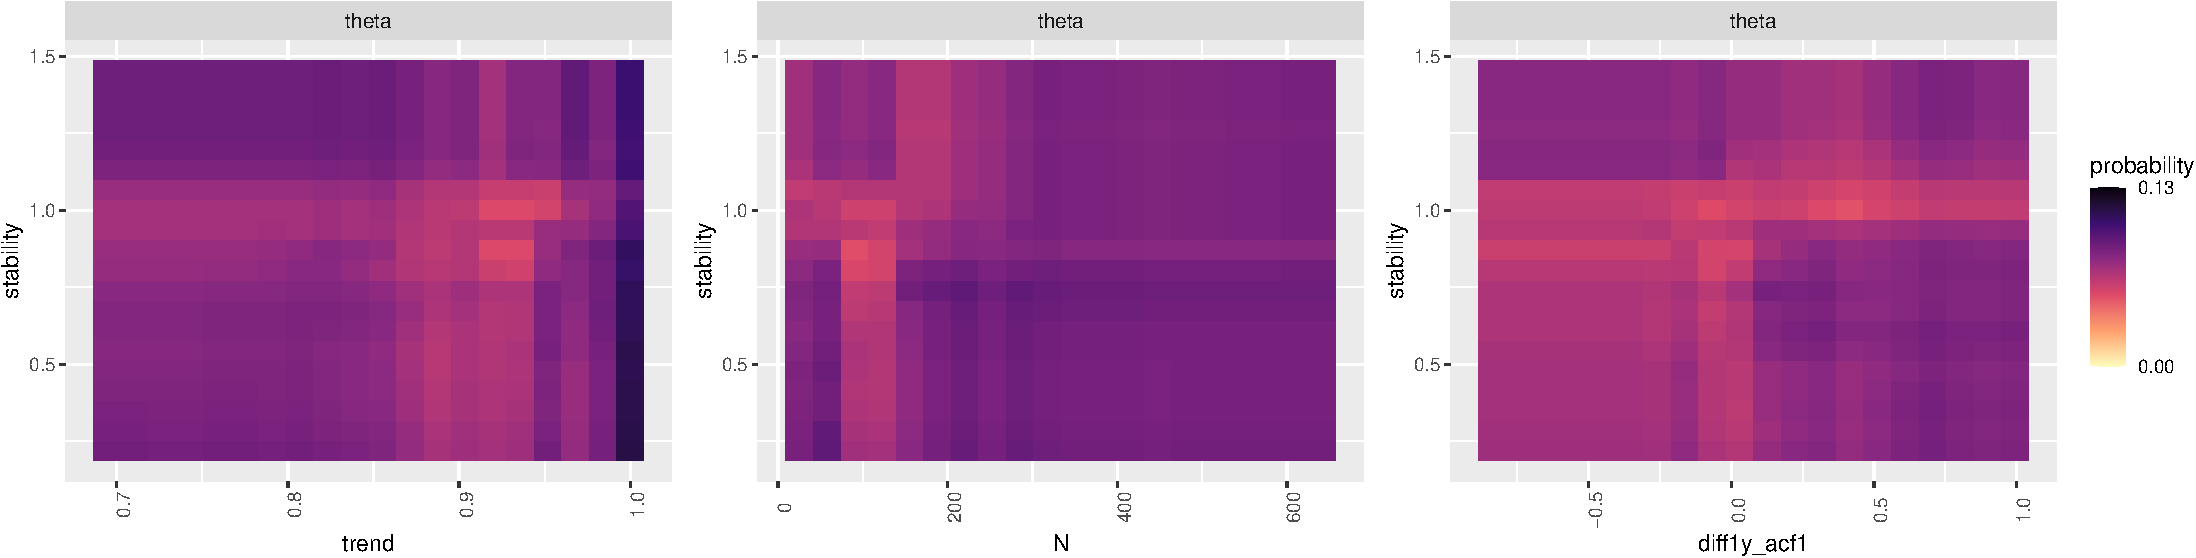
\includegraphics[width=\textwidth]{figure/thetapdp-1} 

}

\caption{Two-way partial dependence plots for linearity for monthly series within theta class. Dark regions show the high probability of belonging to the corresponding class shown in the plot title.}\label{fig:thetapdp}
\end{figure}

\begin{figure}[h]

{\centering 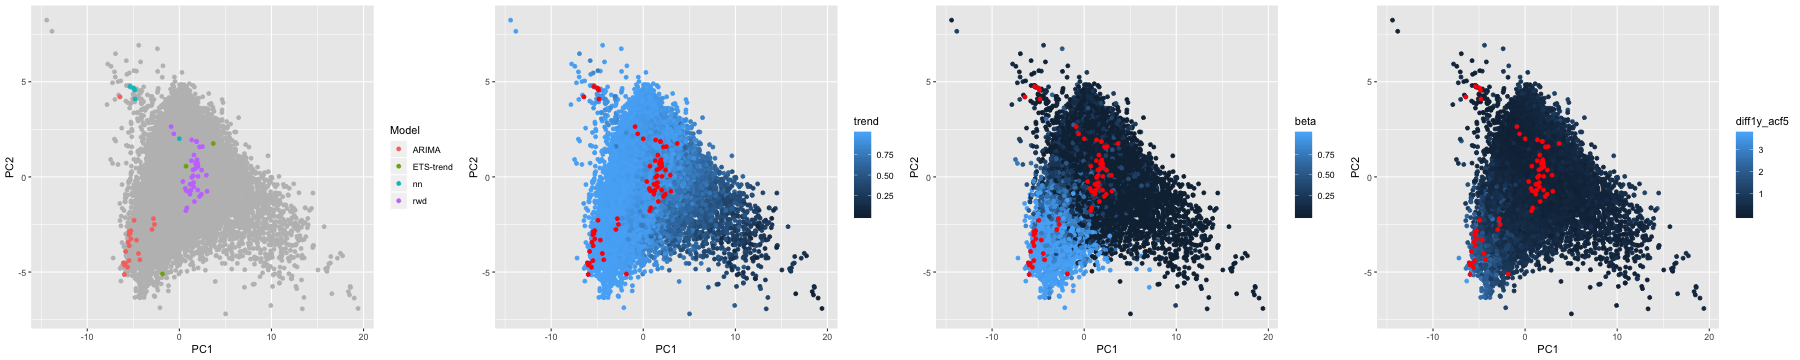
\includegraphics[width=\textwidth]{figure/pcayearly-1} 

}

\caption{Distribution of the yearly time series on the PCA space. On each graph the series that were classified with high probability are highlighted. In the first graph the highlighted points are coloured according to the predicted forecast model. The second, third and forth panels show the distribution of features trend, beta and diff1y\_acf1.  All series that were assigned high voting probability are highly trended.}\label{fig:pcayearly}
\end{figure}

\begin{figure}[h]

{\centering 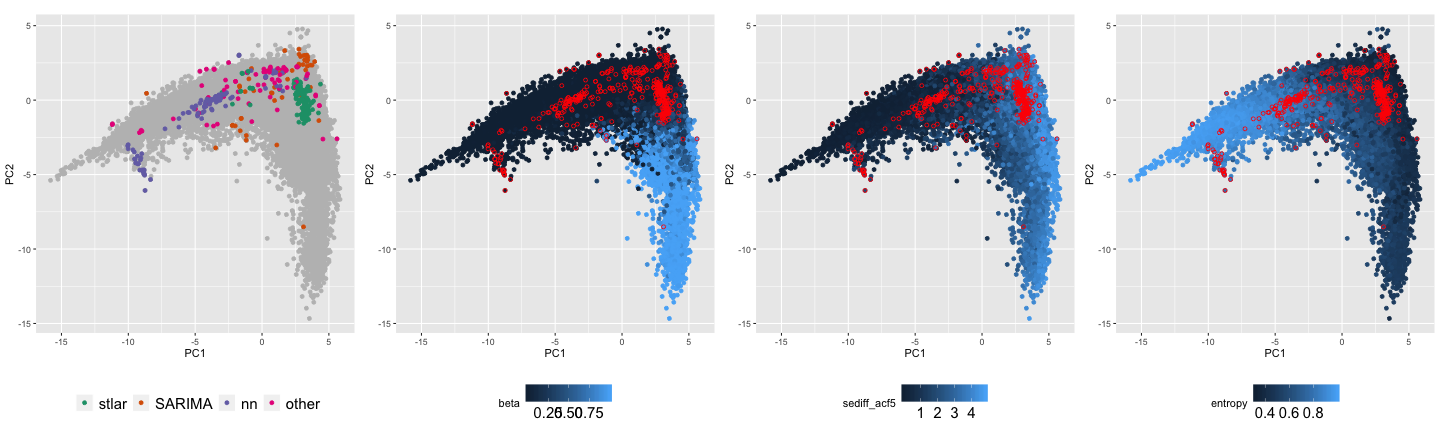
\includegraphics[width=\textwidth]{figure/pcamonthly-1} 

}

\caption{Distribution of the monthly time series on the PCA space. On each graph the series that were classified with high probability are highlighted. In the first graph the highlighted points are coloured according to the predicted forecast model. The second, third and forth panels show the distribution of features beta, sediff\_acf5 and entropy.  The series that are classifed into neural network class with high probability have high entropy value.}\label{fig:pcamonthly}
\end{figure}

\begin{figure}[h]

{\centering 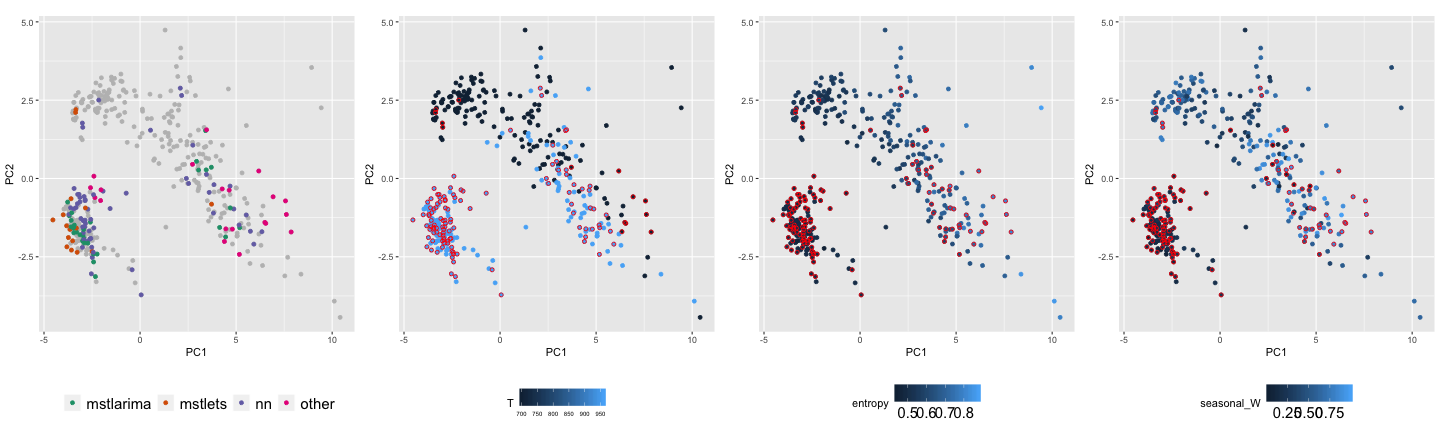
\includegraphics[width=\textwidth]{figure/pcahourly-1} 

}

\caption{Distribution of the hourly time series on the PCA space. On each graph the series that were classified with high probability are highlighted. In the first graph the highlighted points are coloured according to the predicted forecast model. The second, third and forth panels show the distribution of features length, entropy and strength of weekly seasonality. All series that were assigned high voting probability have high value for length.}\label{fig:pcahourly}
\end{figure}

FFORMS framework classified some series with very high probability (greater than 0.6).

\clearpage

\hypertarget{discussion}{%
\section{Discussion and conclusions}\label{discussion}}

In this paper we have proposed a novel framework for forecast-model selection using meta-learning based on time series features. Our proposed FFORMS algorithm uses the knowledge of the past performance of candidate forecast models on a collection of time series in order to identify the best forecasting method for a new series. We have shown that the method almost always performs better than common benchmark methods, and in many cases better than the best-performing methods from both the M1 and the M3 forecasting competitions. Although we have illustrated the method using the M1 and M3 competition data, the framework is general and can be applied to any large collection of time series.

A major advantage of the FFORMS framework is that the classifier is trained offline and selecting a forecasting model for a new time series is as fast as calculating a set of features and passing these to the pretrained classifier. Therefore, unlike traditional model selection strategies or cross-validation processes, our proposed framework can be used to accurately forecast very large collections of time series requiring almost instant forecasts.

In addition to our new FFORMS framework, we have also introduced a simple set of time series features that are useful in identifying the ``best'' forecast method for a given time series, and can be computed rapidly. We will leave to a later study an analysis of which of these features are the most useful, and how our feature set could be reduced further without the loss of forecast accuracy.

For real-time forecasting, our framework involves only the calculation of features, the selection of a forecast method based on the FFORMS random forest classifier, and the calculation of the forecasts from the chosen model. None of these steps involve substantial computation, and they can be easily parallelised when forecasting for a large number of new time series. For future work, we will explore the use of other classification algorithms within the FFORMS algorithm, and test our approach on several other large collections of time series.

\hypertarget{appendix-a-definition-of-features}{%
\section*{Appendix A: Definition of features}\label{appendix-a-definition-of-features}}
\addcontentsline{toc}{section}{Appendix A: Definition of features}

\hypertarget{length-of-time-series}{%
\subsubsection*{Length of time series}\label{length-of-time-series}}
\addcontentsline{toc}{subsubsection}{Length of time series}

The appropriate forecast method for a time series depends on how many observations are available. For example, shorter series tend to need simple models such as a random walk. On the other hand, for longer time series, we have enough information to be able to estimate a number of parameters. For even longer series (over 200 observations), models with time-varying parameters give good forecasts as they help to capture the changes of the model over time.

\hypertarget{features-based-on-an-stl-decomposition}{%
\subsubsection*{Features based on an STL-decomposition}\label{features-based-on-an-stl-decomposition}}
\addcontentsline{toc}{subsubsection}{Features based on an STL-decomposition}

The strength of trend, strength of seasonality, linearity, curvature, spikiness and first autocorrelation coefficient of the remainder series, are calculated based on a decomposition of the time series. Suppose we denote our time series as \(y_1, y_2, \dots,y_T\). First, an automated Box-Cox transformation \autocite{Guerrero1993} is applied to the time series in order to stabilize the variance and to make the seasonal effect additive. The transformed series is denoted by \(y_{t}^*\). For quarterly and monthly data, this is decomposed using STL \autocite{cleveland1990stl} to give \(y_t^*=T_t+S_t+R_t\), where \(T_t\) denotes the trend, \(S_t\) denotes the seasonal component, and \(R_t\) is the remainder component. For non-seasonal data, Friedman's super smoother \autocite{supsmu} is used to decompose \(y_t^*=T_t+R_t\), and \(S_t=0\) for all \(t\). The de-trended series is \(y_t^*-T_t=S_t+R_t\), the deseasonalized series is \(y_t^*-S_t = T_t+R_t\)..

The strength of trend is measured by comparing the variance of the deseasonalized series and the remainder series \autocite{wang2009rule}:
\[
    \text{Trend} = \text{max}\left[0, 1 - \var(R_{t})/\var(T_t+R_t)\right].
\]
Similarly, the strength of seasonality is computed as
\[
    \text{Seasonality} = \text{max}\left[0, 1- \var(R_{t})/ \var(S_t+R_t)\right].
\]

The linearity and curvature features are based on the coefficients of an orthogonal quadratic regression
\[
  T_t=\beta_0+\beta_1 \phi_1(t) + \beta_2\phi_2(t) + \varepsilon_t,
\]
where \(t=1, 2, \dots,T\), and \(\phi_1\) and \(\phi_2\) are orthogonal polynomials of orders 1 and 2. The estimated value of \(\beta_1\) is used as a measure of linearity while the estimated value of \(\beta_2\) is considered as a measure of curvature. These features were used by \textcite{hyndman2015large}. The linearity and curvature depend on the the scale of the time series. Therefore, the time series are scaled to mean zero and variance one before these two features are computed.

The spikiness feature is useful when a time series is affected by occasional outliers. \textcite{hyndman2015large} introduced an index to measure spikiness, computed as the variance of the leave-one-out variances of \(r_t\).

We compute the first autocorrelation coefficient of the remainder series, \(r_t\).

\hypertarget{stability-and-lumpiness}{%
\subsubsection*{Stability and lumpiness}\label{stability-and-lumpiness}}
\addcontentsline{toc}{subsubsection}{Stability and lumpiness}

The features ``stability'' and ``lumpiness'' are calculated based on tiled windows (i.e., they do not overlap). For each window, the sample mean and variance are calculated. The stability feature is calculated as the variance of the means, while lumpiness is the variance of the variances. These were first used by \textcite{hyndman2015large}.

\hypertarget{spectral-entropy-of-a-time-series}{%
\subsubsection*{Spectral entropy of a time series}\label{spectral-entropy-of-a-time-series}}
\addcontentsline{toc}{subsubsection}{Spectral entropy of a time series}

Spectral entropy is based on information theory, and can be used as a measure of the forecastability of a time series. Series that are easy to forecast should have a small spectral entropy value, while very noisy series will have a large spectral entropy. We use the measure introduced by \textcite{goerg2013forecastable} to estimate the spectral entropy. It estimates the Shannon entropy of the spectral density of the normalized spectral density, given by
\[
  H_{s}(y_t):=-\int_{-\pi}^{\pi}\hat f_y(\lambda)\log \hat f_y({\lambda})d\lambda,
\]
where \(\hat{f}_y\) denotes the estimate of the spectral density introduced by \textcite{nuttall1982spectral}. The R package ForeCA \autocite{Foreca} was used to compute this measure.

\hypertarget{hurst-exponent}{%
\subsubsection*{Hurst exponent}\label{hurst-exponent}}
\addcontentsline{toc}{subsubsection}{Hurst exponent}

The Hurst exponent measures the long-term memory of a time series. The Hurst exponent is given by \(H=d+0.5\), where \(d\) is the fractal dimension obtained by estimating a ARFIMA(\(0, d, 0\)) model. We compute this using the maximum likelihood method \autocite{haslett1989space} as implemented in the fracdiff package \autocite{fracdiff}. This measure was also used in \textcite{wang2009rule}.

\hypertarget{nonlinearity}{%
\subsubsection*{Nonlinearity}\label{nonlinearity}}
\addcontentsline{toc}{subsubsection}{Nonlinearity}

To measure the degree of nonlinearity of the time series, we use statistic computed in Terasvirta's neural network test for nonlinearity \autocite{nonlintest}, also used in \textcite{wang2009rule}. This takes large values when the series is nonlinear, and values around 0 when the series is linear.

\hypertarget{parameter-estimates-of-an-ets-model}{%
\subsubsection*{Parameter estimates of an ETS model}\label{parameter-estimates-of-an-ets-model}}
\addcontentsline{toc}{subsubsection}{Parameter estimates of an ETS model}

The ETS (A,A,N) model \autocite{expsmooth08} produces equivalent forecasts to Holt's linear trend method, and can be expressed as follows:
\begin{align*}
  y_t    & = \ell_{t-1}+b_{t-1}+\varepsilon_t\\
  \ell_t & = \ell_{t-1}+b_{t-1}+\alpha \varepsilon_t\\
  b_t    & = b_{t-1}+\beta \varepsilon_t,
\end{align*}
where \(\alpha\) is the smoothing parameter for the level, and \(\beta\) is the smoothing parameter for the trend. We include the parameter estimates of both \(\alpha\) and \(\beta\) in our feature set for yearly time series. These indicate the variability in the level and slope of the time series.

The ETS(A,A,A) model \autocite{expsmooth08} produces equivalent forecasts to Holt-Winters' additive method, and can be expressed as follows:
\begin{align*}
  y_t    & = \ell_{t-1}+b_{t-1}+s_{t-m}+\varepsilon_t\\
  \ell_t & = \ell_{t-1}+b_{t-1}+s_{t-m}+\alpha \varepsilon_t\\
  b_t    & = b_{t-1}+\beta \varepsilon_t,\\
  s_t &= s_{t-m} + \gamma\varepsilon_t,
\end{align*}
where \(\gamma\) is the smoothing parameter for the seasonal component, and the other parameters are as above. We include the parameter estimates of \(\alpha\), \(\beta\) and \(\gamma\) in our feature set for monthly and quarterly time series. The value of \(\gamma\) provides a measure for the variability of the seasonality of a time series.

\hypertarget{unit-root-test-statistics}{%
\subsubsection*{Unit root test statistics}\label{unit-root-test-statistics}}
\addcontentsline{toc}{subsubsection}{Unit root test statistics}

The Phillips-Perron test is based on the regression \(y_t= c + \alpha y_{t-1}+ \varepsilon_t\). The test statistic we use as a feature is the usual ``Z-alpha'' statistic with the Bartlett window parameter set to the integer value of \(4(T/100)^{0.25}\) \autocite{Pfaff2008}. This is the default value returned from the \texttt{ur.pp()} function in the \texttt{urca} package \autocite{pfaff2016package}.

The KPSS test is based on the regression \(y_t=c+\delta t+\alpha y_{t-1}+\varepsilon_t\). The test statistic we use as a feature is the usual KPSS statistic with the Bartlett window parameter set to the integer value of \(4(T/100)^{0.25}\) \autocite{Pfaff2008}. This is the default value returned from the \texttt{ur.kpss()} function in the \texttt{urca} package \autocite{pfaff2016package}.

\hypertarget{autocorrelation-coefficient-based-features}{%
\subsubsection*{Autocorrelation coefficient based features}\label{autocorrelation-coefficient-based-features}}
\addcontentsline{toc}{subsubsection}{Autocorrelation coefficient based features}

We calculate the first-order autocorrelation coefficient and the sum of squares of the first five autocorrelation coefficients of the original series, the first-differenced series, the second-differenced series, and the seasonally differenced series (for seasonal data).

A linear trend model is fitted to the time series, and the first-order autocorrelation coefficient of the residual series is calculated.

We calculate the sum of squares of the first five partial autocorrelation coefficients of the original series, the first-differenced series and the second-differenced series.

\printbibliography

\end{document}
